\chapter{Эпитаксиальные наночастицы GaAs}\label{ch:ch5}

GaAs~--- третий по масштабам использования в полупроводниковой промышленности
материал после кремния и германия. В последнее десятилетие разработано
несколько важных приложений на основе синтезированных на Si наноструктур GaAs:
солнечные элементы \cite{Chu2014}, активный слой для оптоэлектронных устройств
\cite{Bietti2009}, структура металл\,--\,оксид\,--\,полупроводник
\cite{Zhao2009}, однофотонный излучатель \cite{Sanguinetti2015}.

В этой главе излагается результат исследований формирования методом МПЭ и
оптических свойств эпитаксиальных наночастиц GaAs на подложках Si(111) без
поверхностного оксида. Показано, что GaAs может образовывать огранённые
наночастицы, окружённые сплошным слоем сросшихся островков GaAs. Исследовано
влияние условий синтеза на морфологию наноструктур.

\section{Постановка эксперимента}\label{sec:ch5/sec1}

Наноструктуры GaAs синтезированы на установке МПЭ Veeco GEN III на подложках
Si(111). Перед загрузкой в установку подложки химически обрабатывались
последовательным кипячением в растворах CCl\textsubscript{4}, изопропанола и
растворе
NH\textsubscript{4}OH:H\textsubscript{2}O\textsubscript{2}:H\textsubscript{2}O
в соотношении 1:1:3, естественный поверхностный оксид удалялся погружением в
1:10 раствор HF:H\textsubscript{2}O с последующим промыванием в
деионизированной воде. После загрузки в установку подложки дегазировали в
промежуточной камере при температуре 400~\si{\degreeCelsius}. В ростовой камере
подложка нагревалась до температуры роста без предварительного
высокотемпературного отжига.

Рост начинался одновременной подачей молекулярных потоков Ga и
As\textsubscript{4}. Во время роста всех исследуемых образцов поток Ga
поддерживался постоянным и соответствовал планарной скорости роста
GaAs/GaAs(001) равной 0,4~\si{\micro\metre\per\hour} в избытке As. При
обсуждении поток As\textsubscript{4} в работе используются относительные
единицы, за единицу которых взят «стехиометрический» поток~--- абсолютный поток
As\textsubscript{4} при котором в сочетании с потоком Ga, который соответствует
планарной скорости роста GaAs/GaAs(001) равной 0,4~\si{\micro\metre\per\hour} в
избытке As, достигается стехиометрическое отношение адатомов на поверхности
GaAs, определяемое по фазовому переходу от As-обогащённой реконструкции
GaAs\((001)4\)\(\times\)\(2\) к Ga-обогащённой GaAs\((001)2\)\(\times\)\(4\)
при температуре подложки 550~\si{\degreeCelsius} во время роста планарного
GaAs/GaAs(001). Данный переход наблюдается при отношении ЭДП
As\textsubscript{4}/Ga \(\approx 12\). Данные условия роста приводят к
образованию одиночных наночастиц GaAs, окружённых шероховатым сплошным слоем.

Морфология синтезированных наногетероструктур изучена методом PЭМ (Zeiss SUPRA
25) и АСМ (Bruker Bioscope Catalyst SPM). Изображения АСМ обработаны в
программе Gwyddion. Спектры КРС и ФЛ получены при комнатной температуре
(300~\si{\kelvin}), используя лазерное возбуждение с длиной волны
532~\si{\nano\metre} на спектрометре Horiba LabRam HR800. Спектрометр совмещён
с пьезодвигателем, позволяющим проводить измерения в геометрии обратного
рассеяния с пространственным разрешением менее 0,5~\si{\micro\metre}, и
оптическим конфокальным микроскопом Olympus IX71 с объективом Olympus Plan N
100\(\times\)/0,95~NA.

\section{Обсуждение экспериментальных результатов}\label{sec:ch5/sec2}

\subsection{Влияние ростовых параметров на морфологию
наноструктур}\label{subsec:ch5/sec2/sub1}

Для исследования влияния условий роста на морфологию наночастиц GaAs
синтезированы образцы при различных ЭДП As и ростовых температурах подложки с
сохранением постоянного потока Ga. Влияние изменения соотношения молекулярных
потоков As/Ga было изучено на основе образцов, выращенных при температуре
подложки 550~\si{\degreeCelsius}, потоке As в 2, 4 и 6~отн.~ед.

На поверхности подложки вокруг эпитаксиальных наночастиц GaAs отсутствует
синтезированный материал, на РЭМ изображениях эта область имеет тёмный контраст
(см.~рис.~\cref{fig:Image_31}). Можно предположить, что наночастицы могут
зарождаться на неоднородностях поверхности подложки: на островках
SiO\textsubscript{x}, образующихся до загрузки подложек в установку МПЭ
\cite{Miura1996, Ogawa1996}, или шероховатостях из-за неоднородного окисления
подложки и последующего травления в HF \cite{Neuwald1992, Jakob1991}. Адатомы
Ga накапливается на этих участках с последующим формированием наночастиц GaAs в
режиме ПЖК \cite{Dubrovskii2012a}, а обычный трёхмерный рост в режиме
пар\,--\,кристалл с высокой поверхностной плотностью зарождения происходит на
свободной поверхности Si(111).

\begin{figure}[ht] \centerfloat{ \subcaptionbox{\label{fig:Image_31_1}}{%
			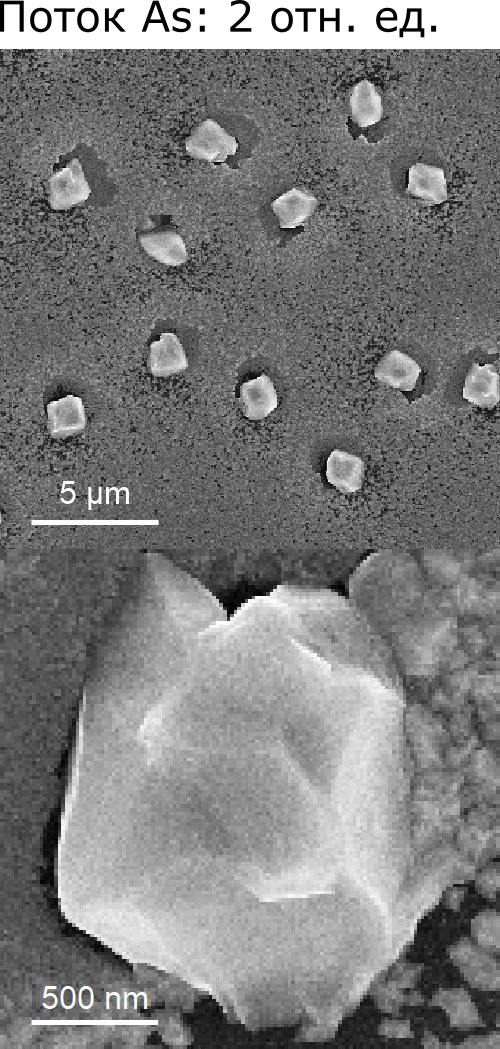
\includegraphics[width=0.25\linewidth]{Image_31_1}}
			\subcaptionbox{\label{fig:Image_31_2}}{%
				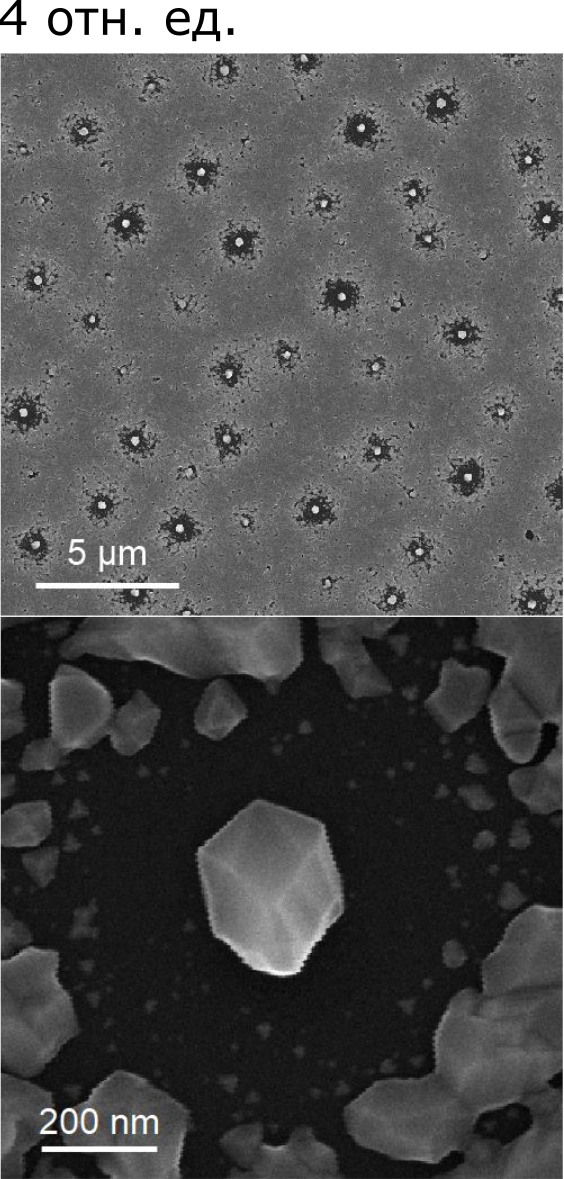
\includegraphics[width=0.25\linewidth]{Image_31_2}}
				\subcaptionbox{\label{fig:Image_31_3}}{%
				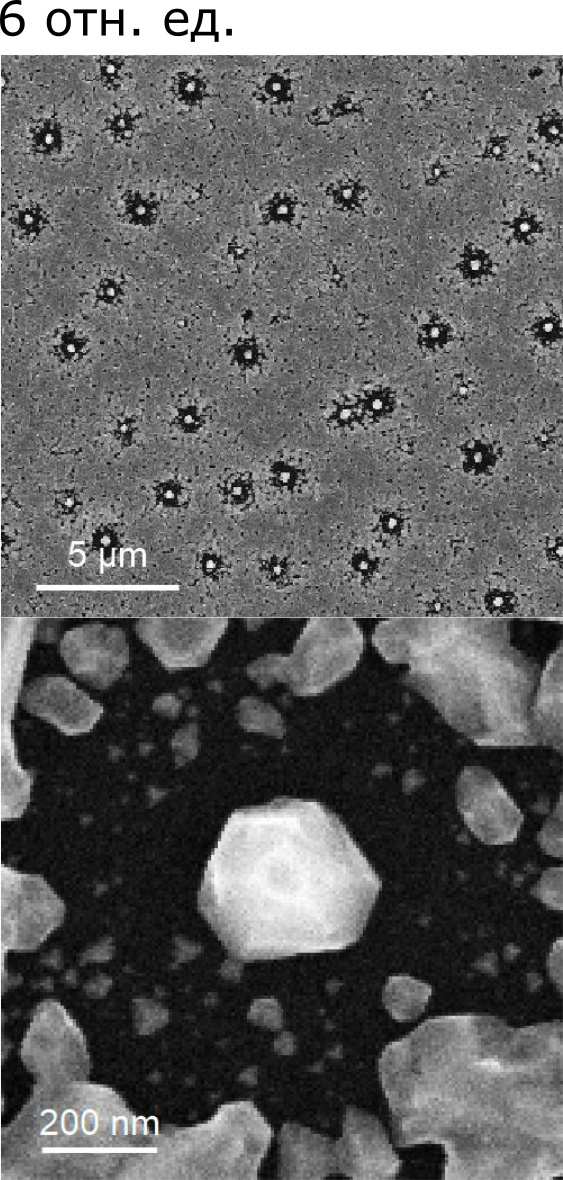
\includegraphics[width=0.25\linewidth]{Image_31_3}} } \legend{Поток As:
				2 (а), 4 (б) и 6~отн.~ед (в) (температура роста
				550~\si{\degreeCelsius})} \caption{РЭМ изображения наноструктур GaAs,
				синтезированных при различных потоках As}\label{fig:Image_31}
			\end{figure}

Результаты анализа влияния соотношения молекулярных потоков As/Ga на морфологию
наночастиц представлены на рисунках~\cref{fig:tab_2} и ~\cref{fig:tab_2_3}. При
низком соотношении потоков As/Ga (поток As 2~отн.~ед.) формируется самая низкая
поверхностная плотность массива наночастиц, наибольший латеральный размер и
высота наночастиц. Увеличение соотношения потоков As/Ga (увеличение потока As с
2 до 4~отн.~ед.) приводит к трёхкратному увеличению поверхностной плотности
массива наночастиц и резкому уменьшению их латерального размера (с \(\approx
1900\)~\si{\nano\metre} до \(\approx 250\)~\si{\nano\metre}). Дальнейшее
увеличение соотношения потоков As/Ga (увеличение потока As с 4 до 6~отн.~ед.)
оказывает слабое влияние на морфологию наночастиц и сплошного слоя, что
указывает на переход к режиму ограничения скорости роста потоком Ga.

\begin{figure}[ht] \centerfloat{ \subcaptionbox{\label{fig:tab_2_1}}{%
			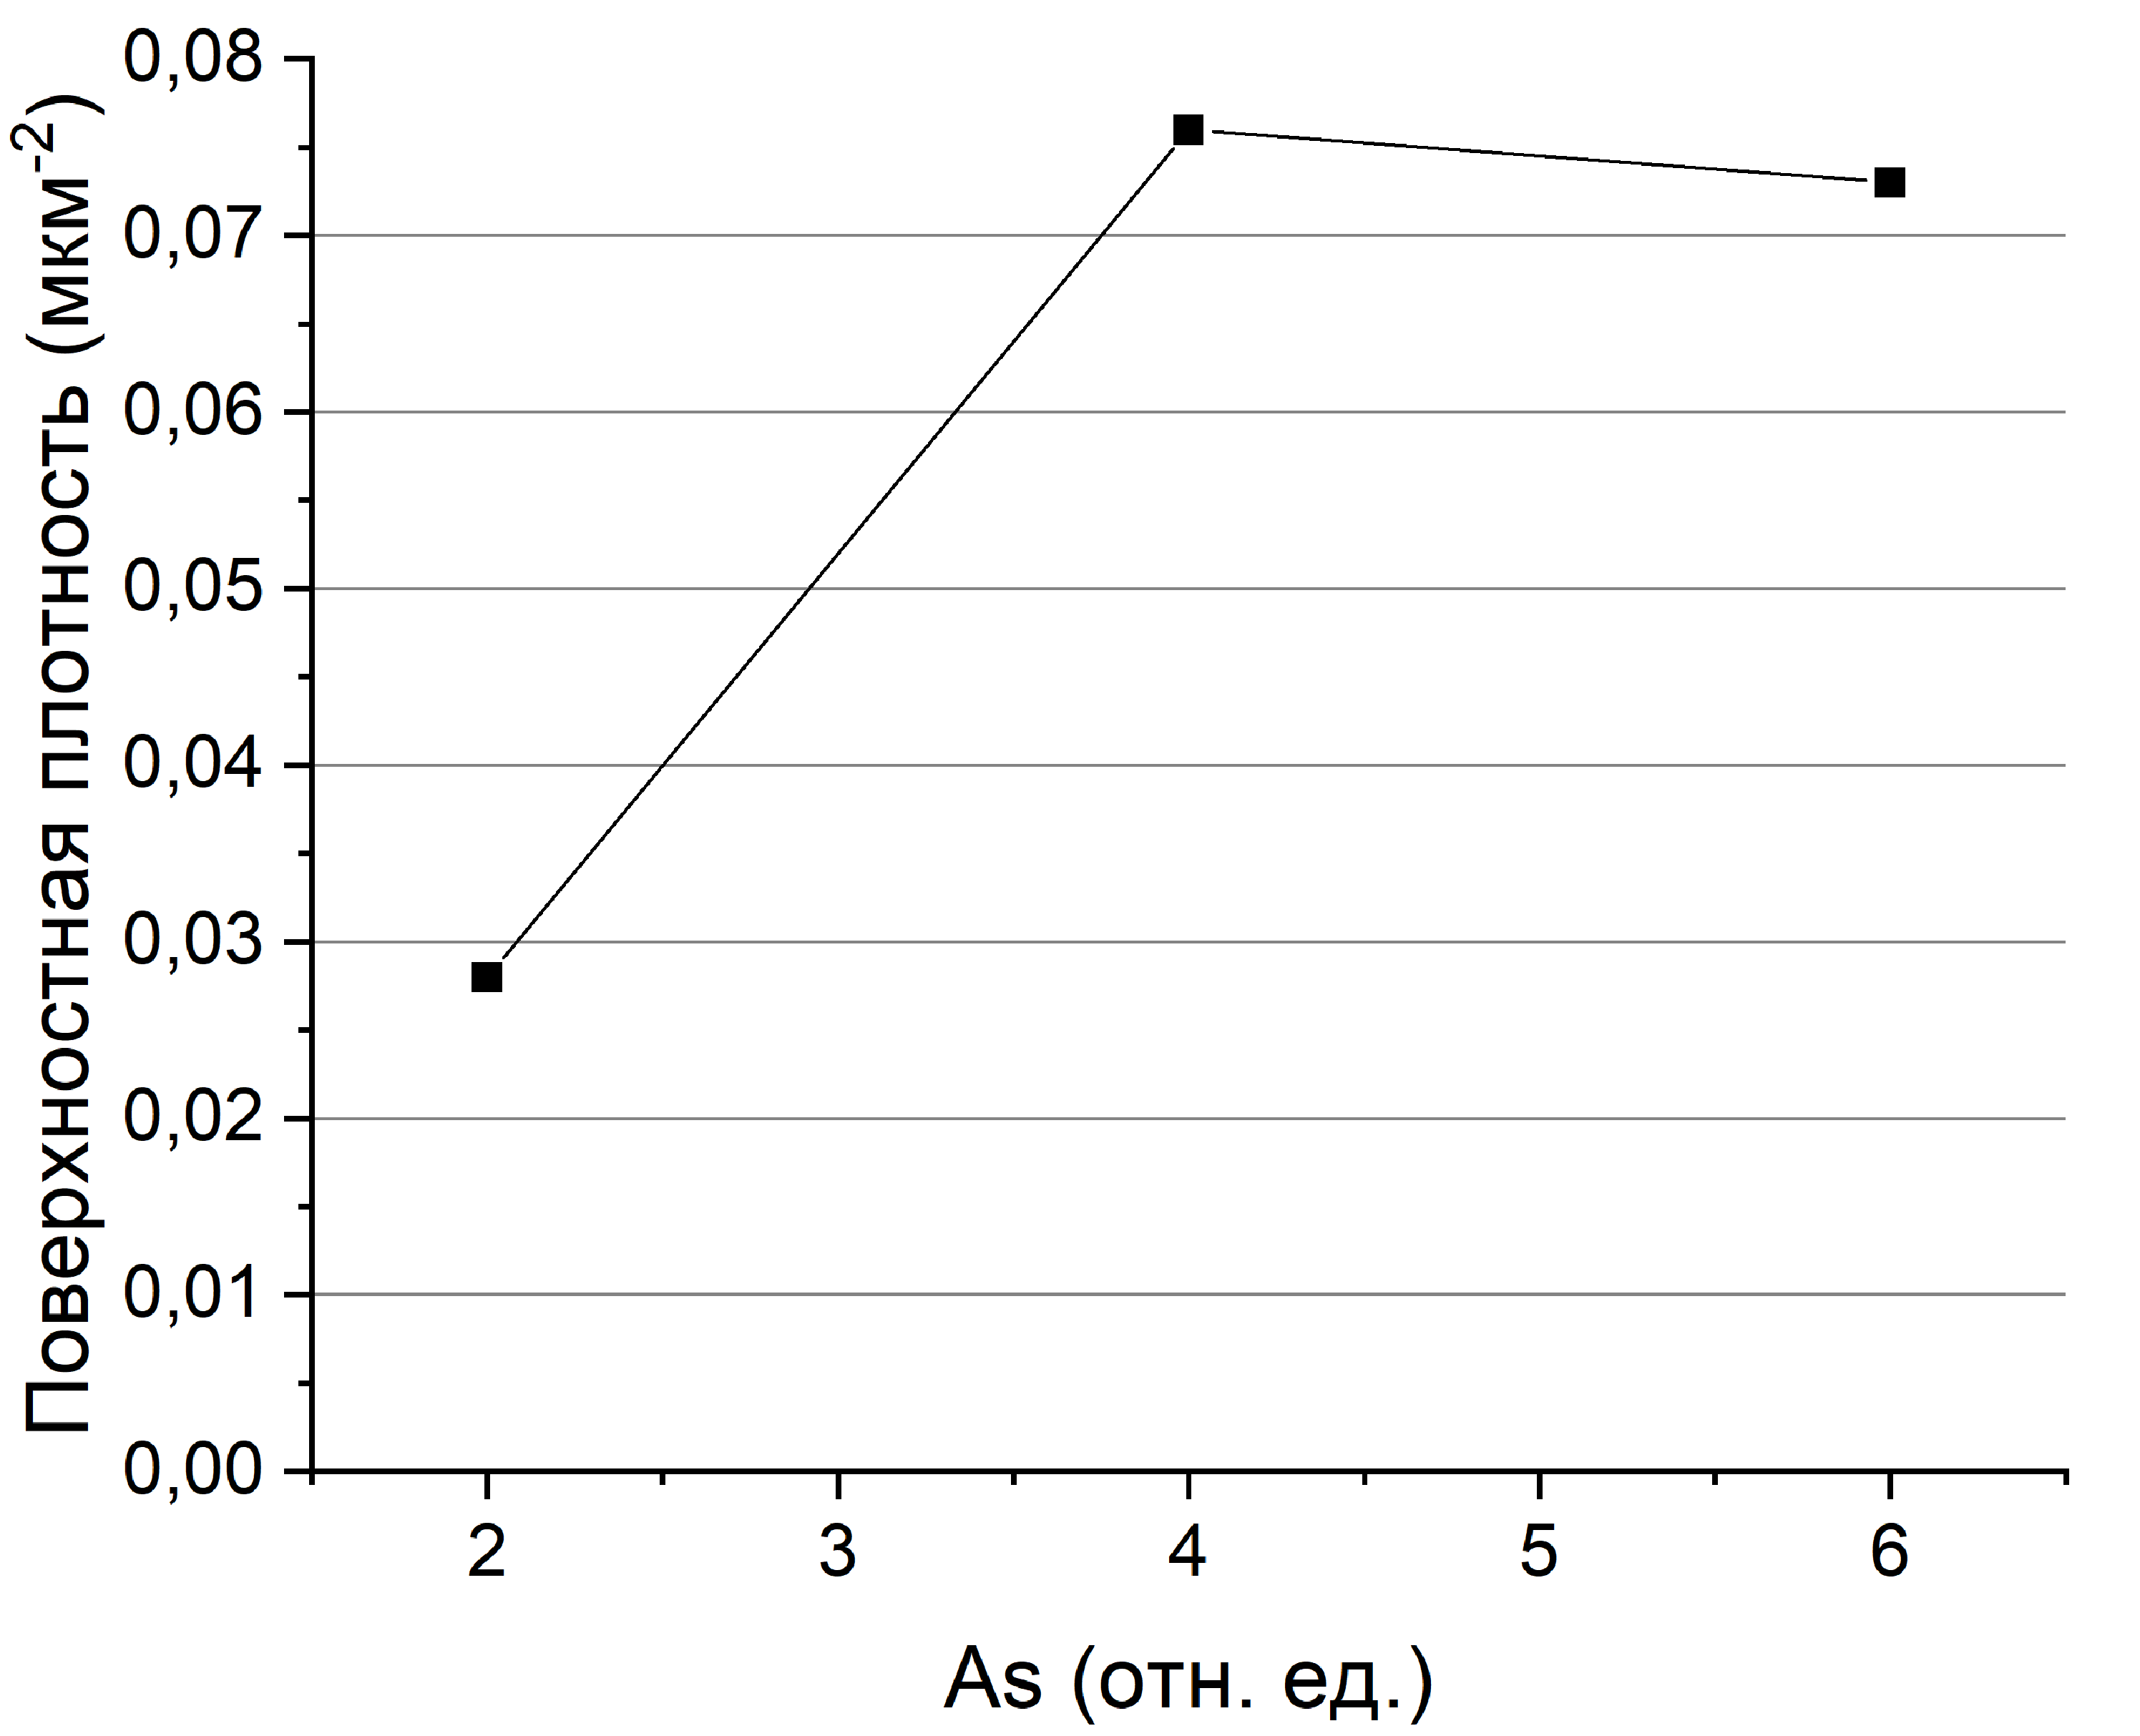
\includegraphics[width=0.48\linewidth]{tab_2_1}}
			\subcaptionbox{\label{fig:tab_2_2}}{%
			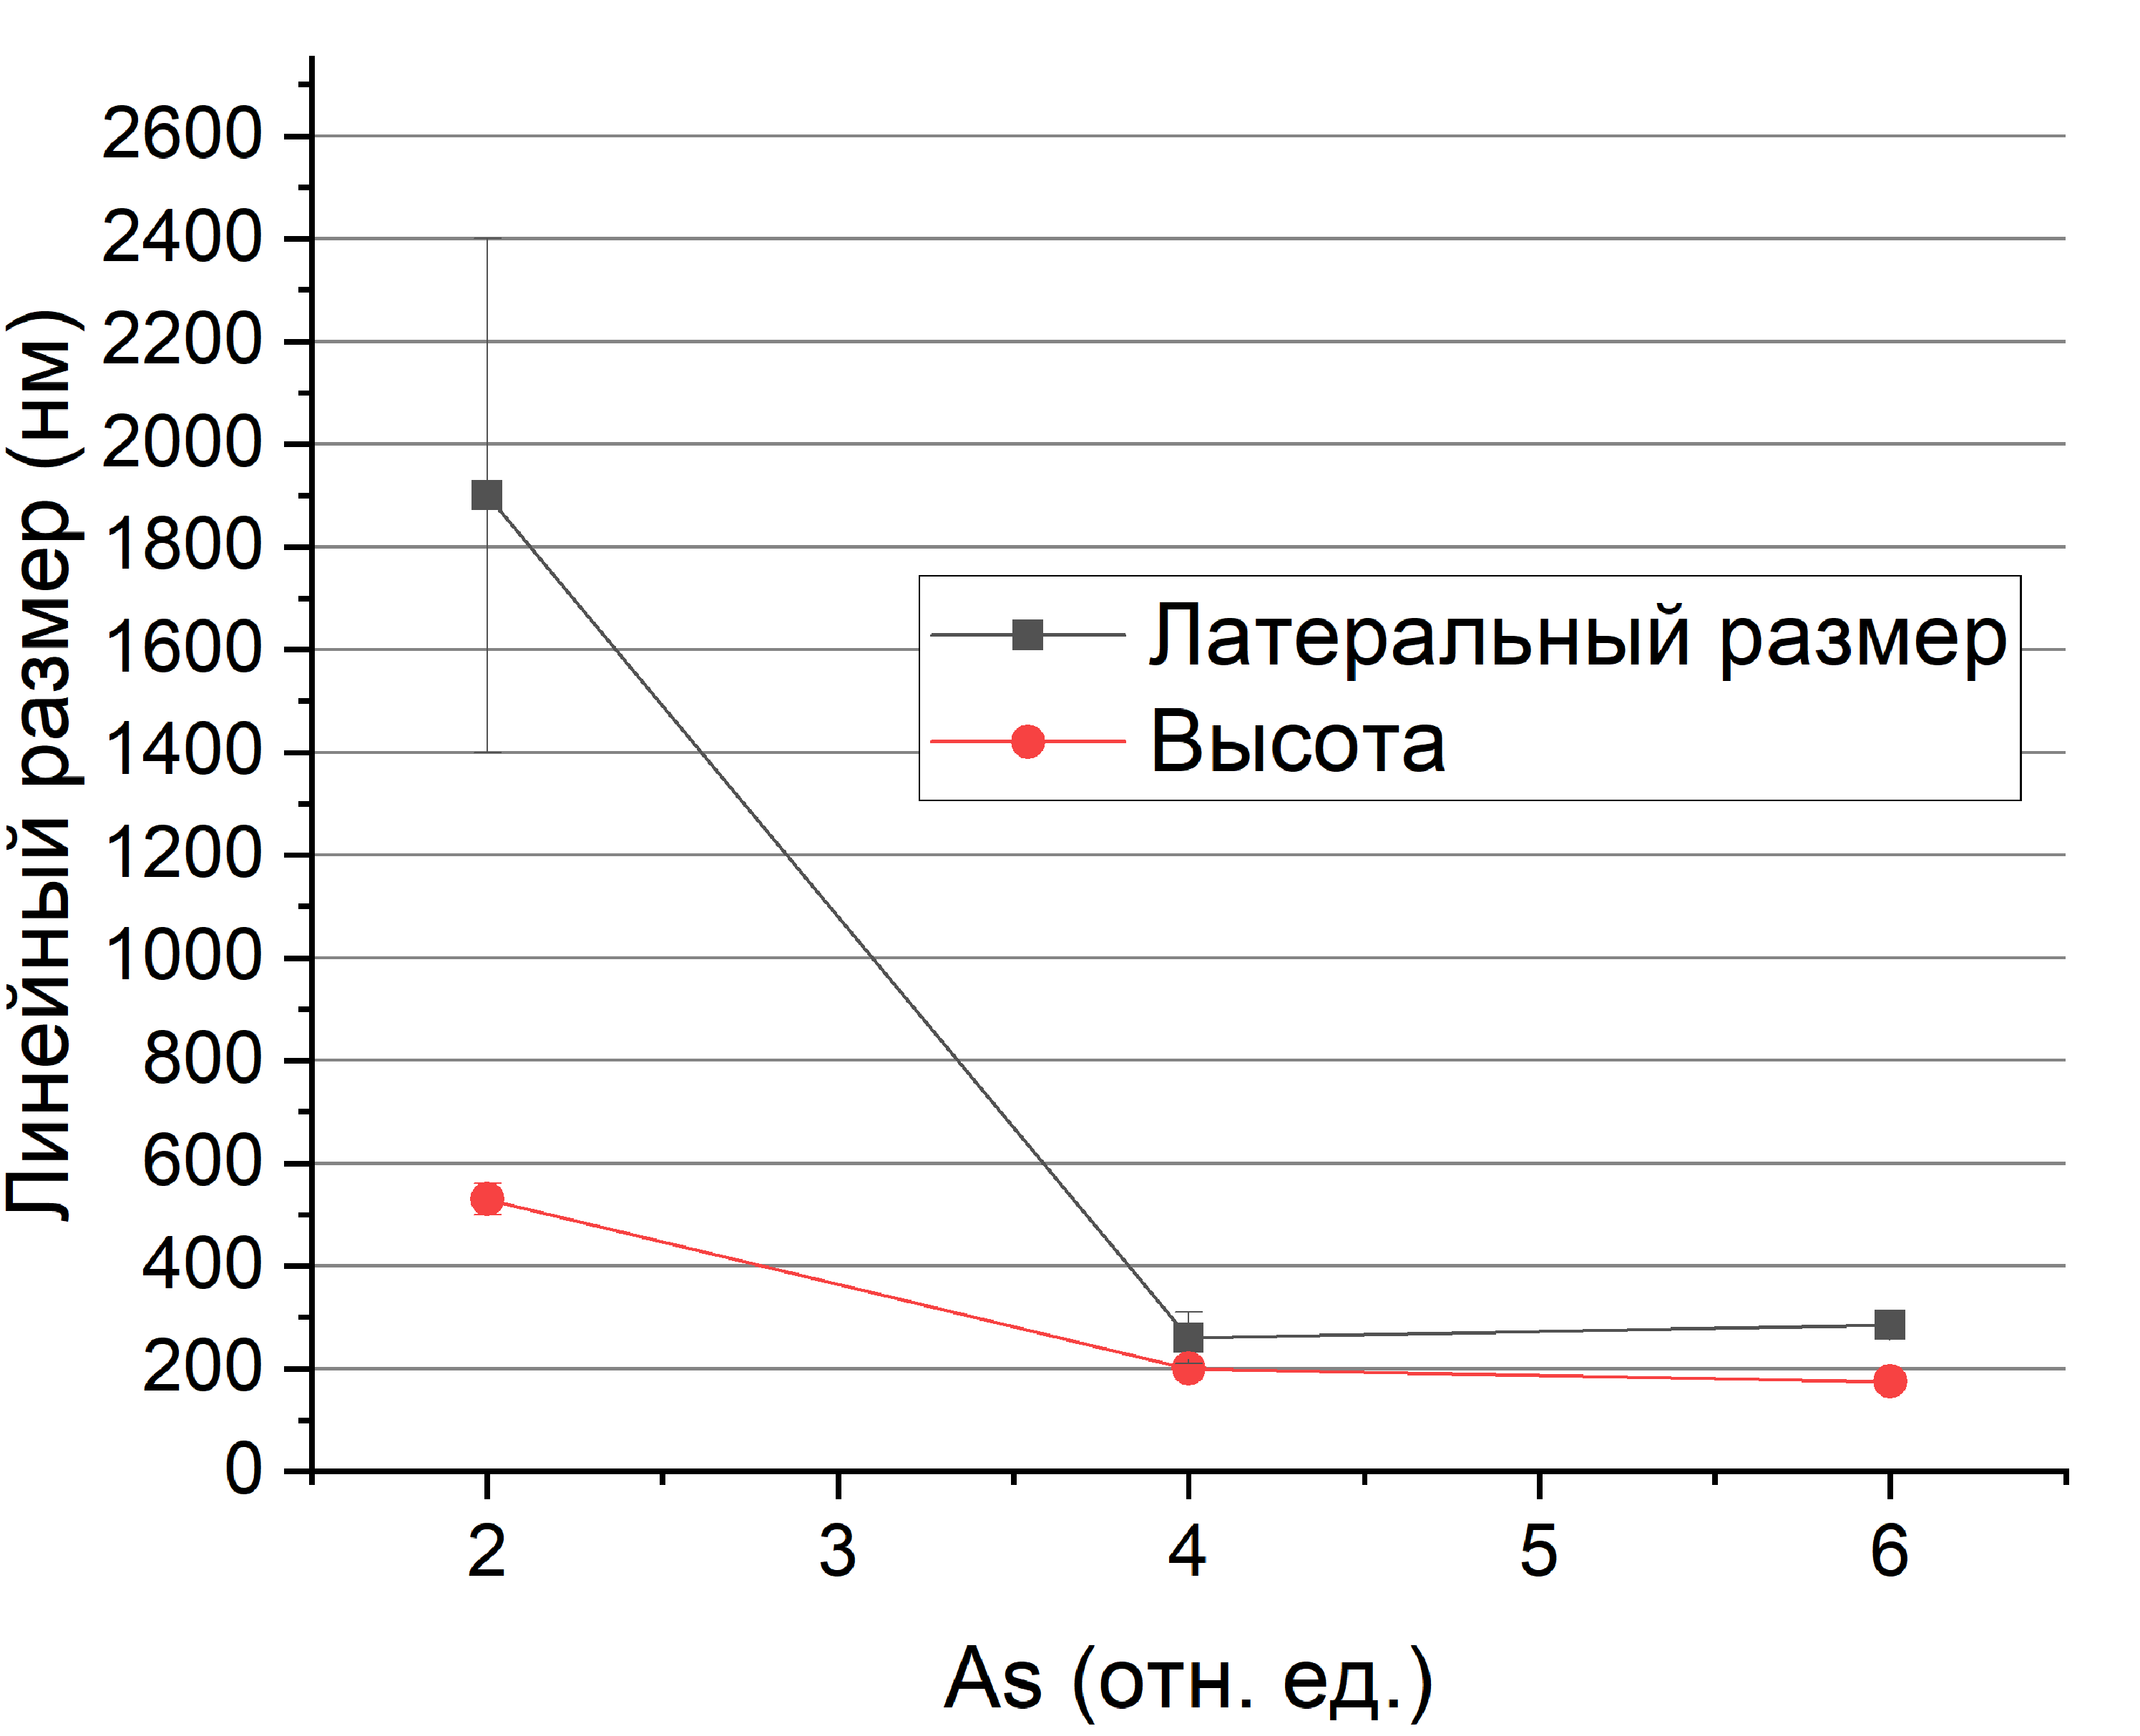
\includegraphics[width=0.48\linewidth]{tab_2_2}} } \legend{Наноструктуры
			GaAs синтезированы при температуре подложки 550~\si{\degreeCelsius}}
			\caption{Зависимости поверхностной плотности массива~(а) и линейных
				размеров наночастиц~(б)  от соотношения потоков As/Ga}\label{fig:tab_2}
			\end{figure}

\begin{figure}[ht] \centerfloat{
		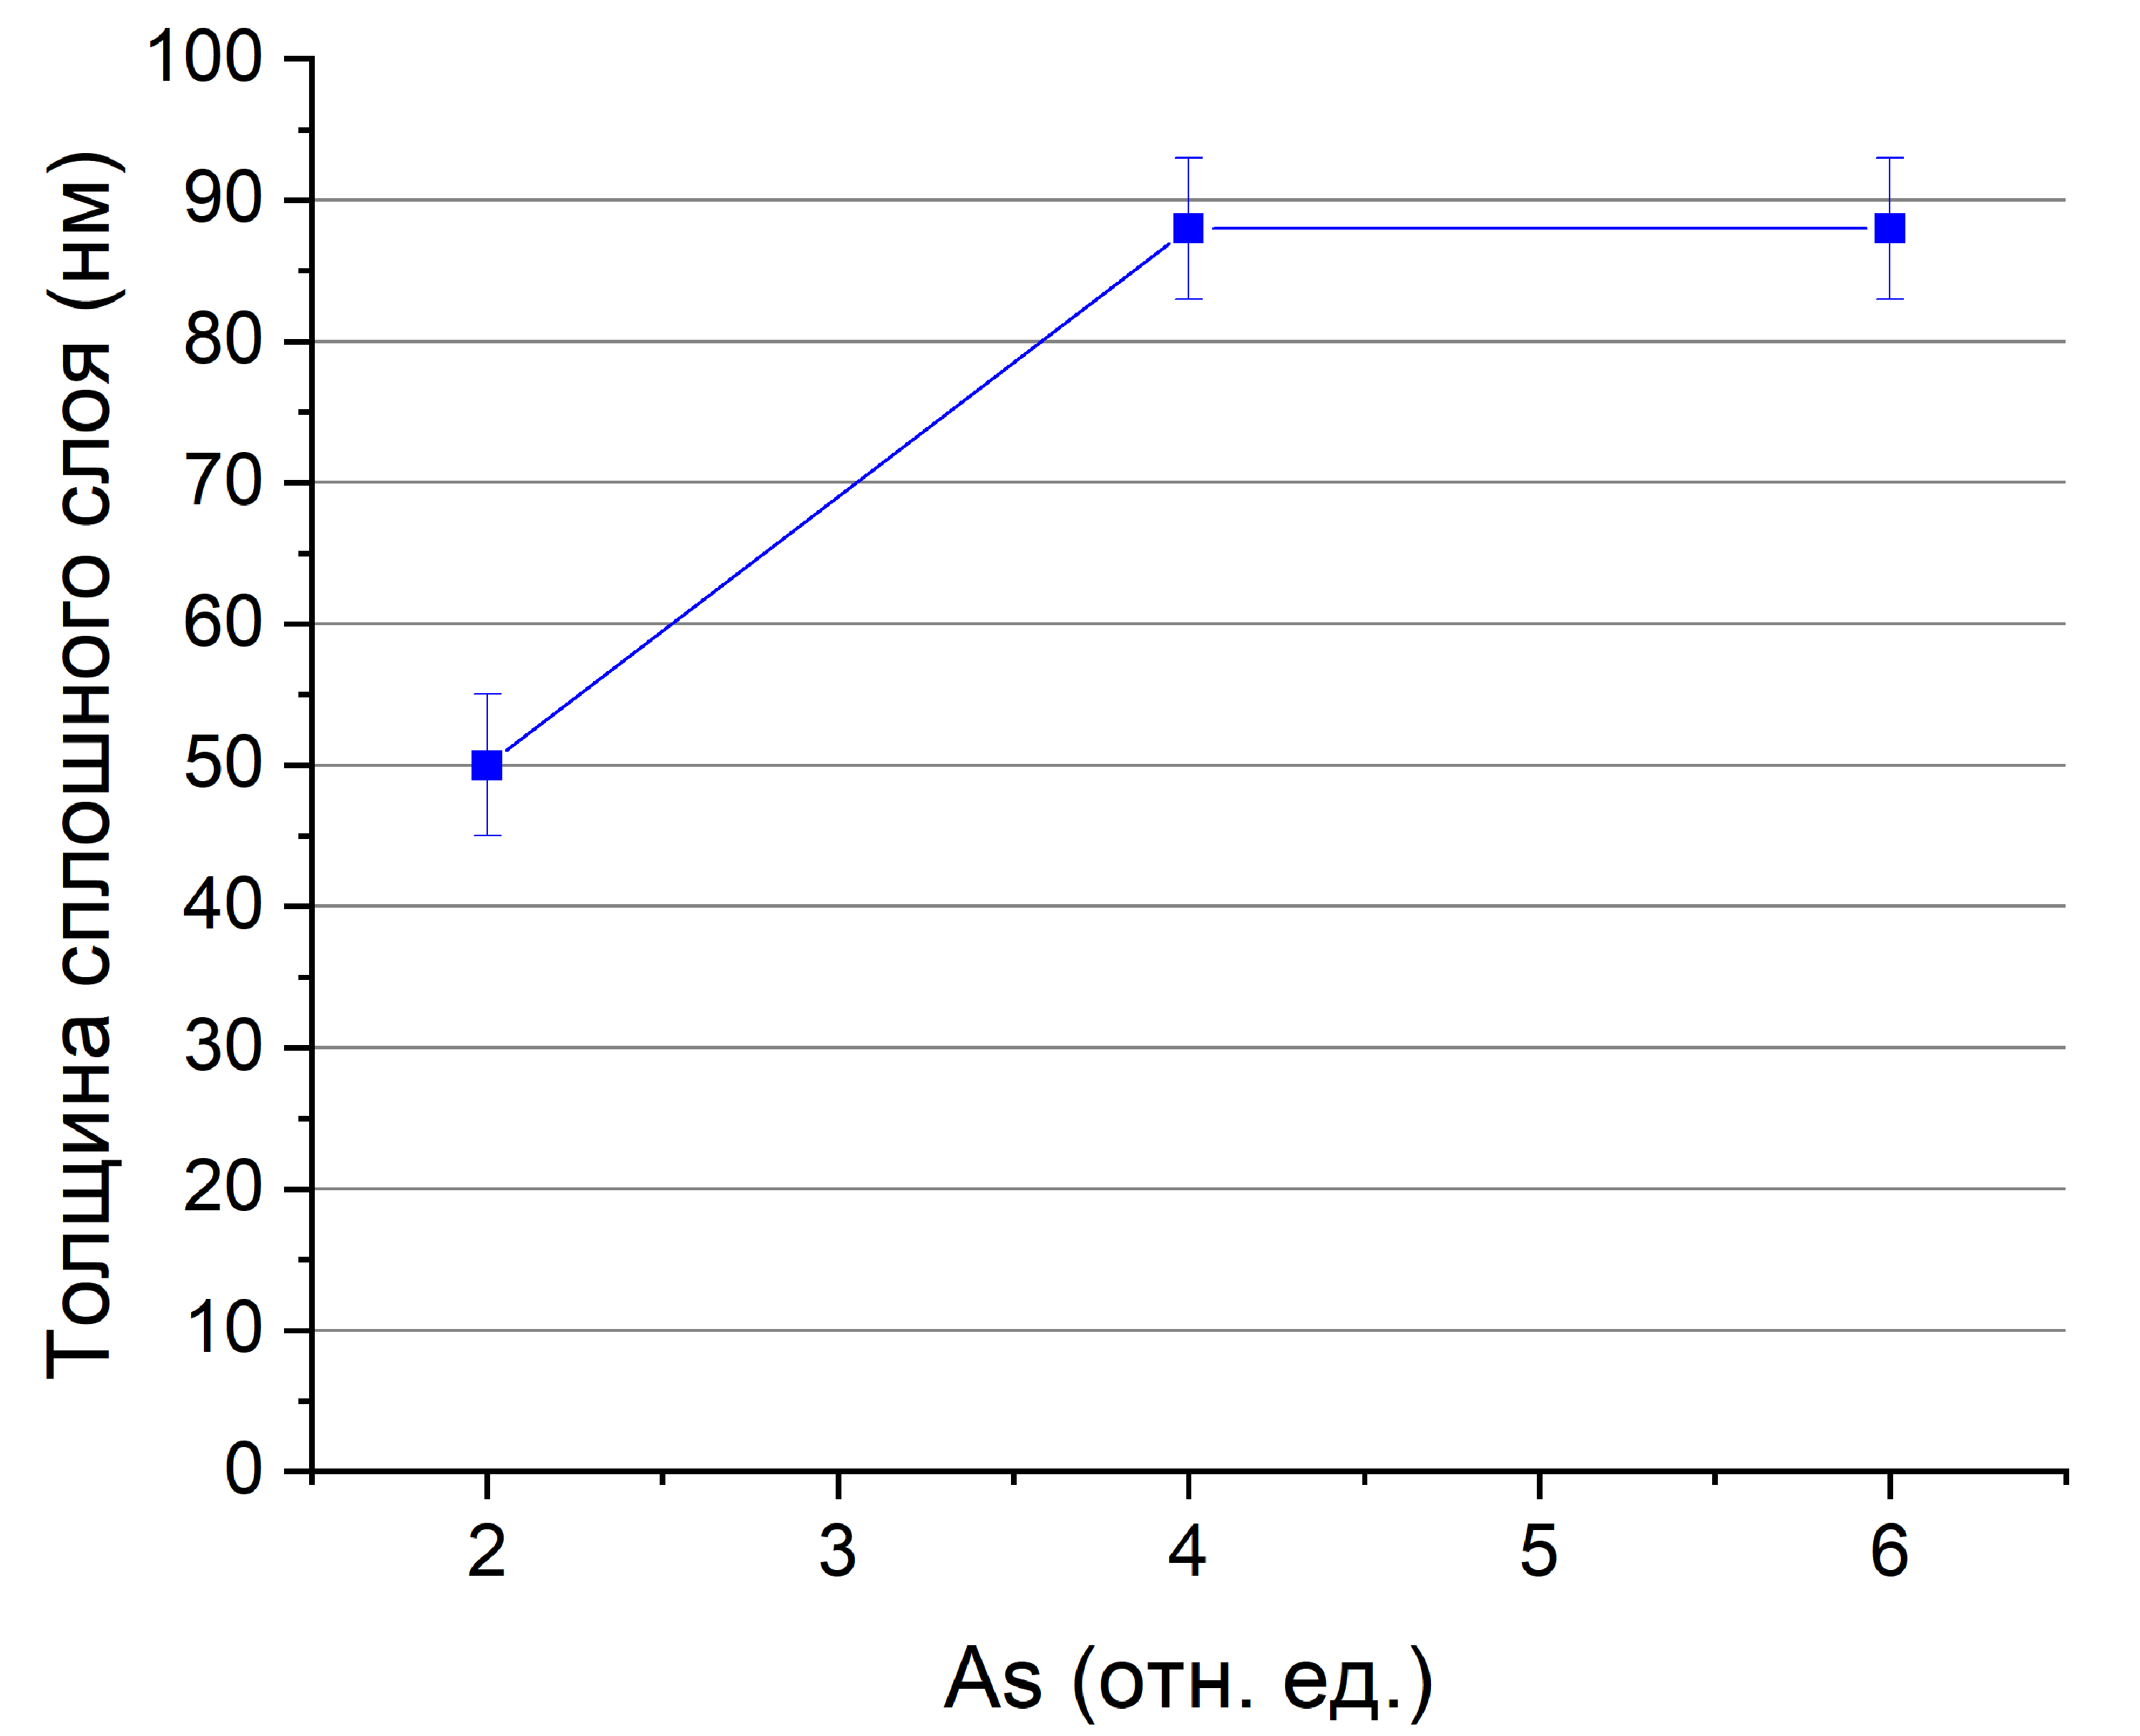
\includegraphics[width=0.48\linewidth]{tab_2_3} } \legend{Наноструктуры
		GaAs синтезированы при температуре подложки 550~\si{\degreeCelsius}}
		\caption{Зависимость толщины сплошного слоя от соотношения потоков
	As/Ga}\label{fig:tab_2_3} \end{figure}

Влияние соотношения потоков As/Ga на морфологию наночастиц вызвано подавлением
диффузии адатомов Ga адатомами V группы. Снижение потока As ниже 2~отн.~ед.
может привести к накоплению капель Ga, а увеличение~--- подавить диффузию
частиц Ga, что увеличивает поверхностную плотность наночастиц и способствует
росту сплошного слоя.

Другой контролируемый ростовой параметр~--- температура подложки. Для
исследования его влияния была синтезирована серия образцов при температуре
роста от 550 до 630~\si{\degreeCelsius} и потоке As в 4~отн.~ед.
(см.~рис.~\cref{fig:Image_32}).

\begin{figure}[ht] \centerfloat{ \subcaptionbox{\label{fig:Image_32_1}}{%
			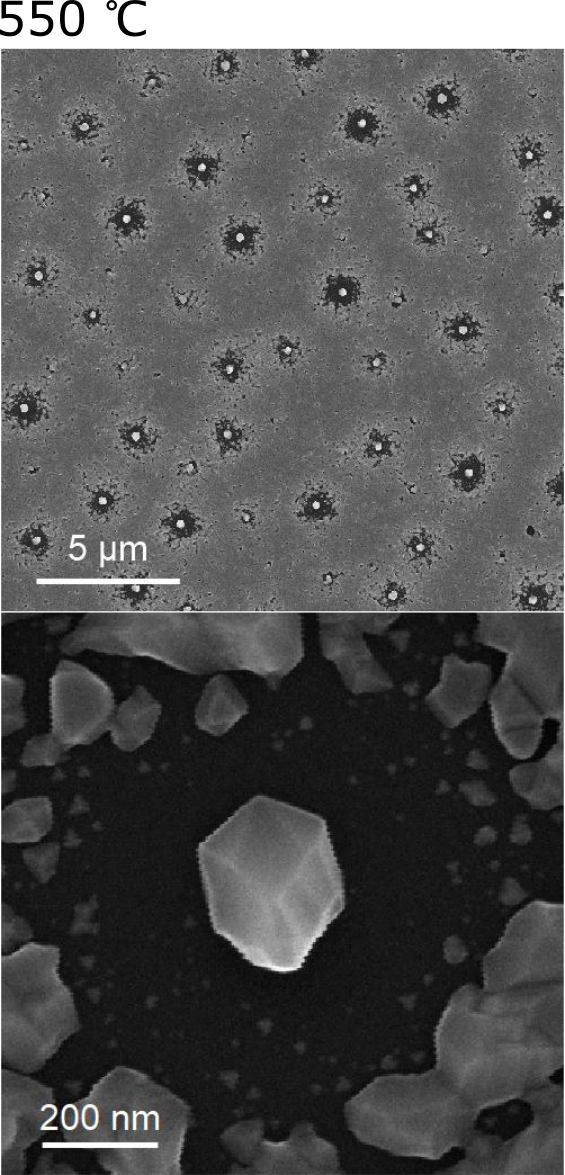
\includegraphics[width=0.25\linewidth]{Image_32_1}}
			\subcaptionbox{\label{fig:Image_32_2}}{%
				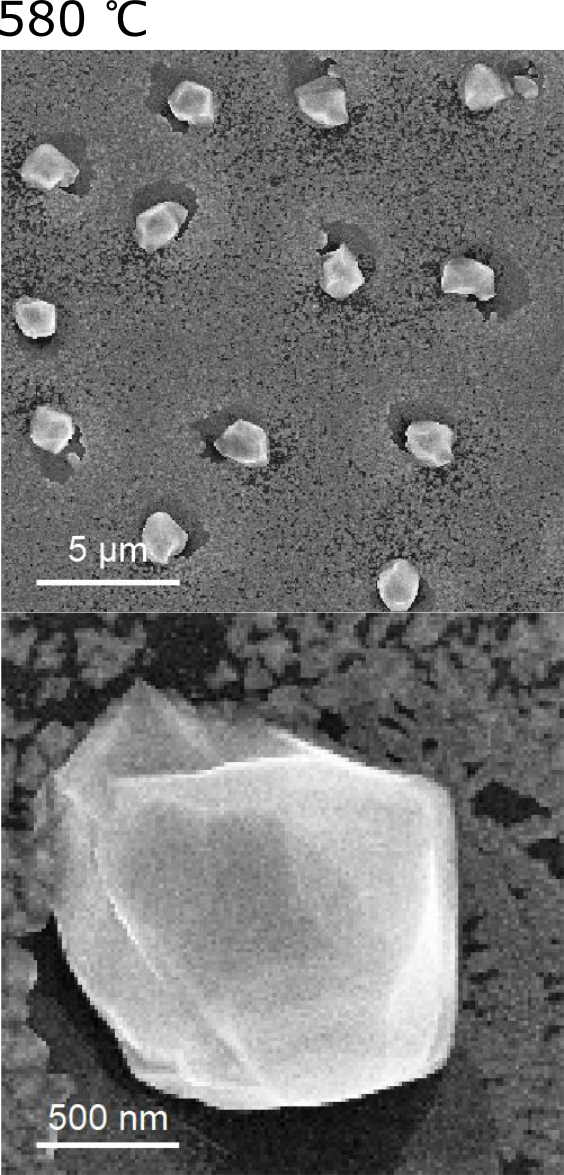
\includegraphics[width=0.25\linewidth]{Image_32_2}}
				\subcaptionbox{\label{fig:Image_32_3}}{%
				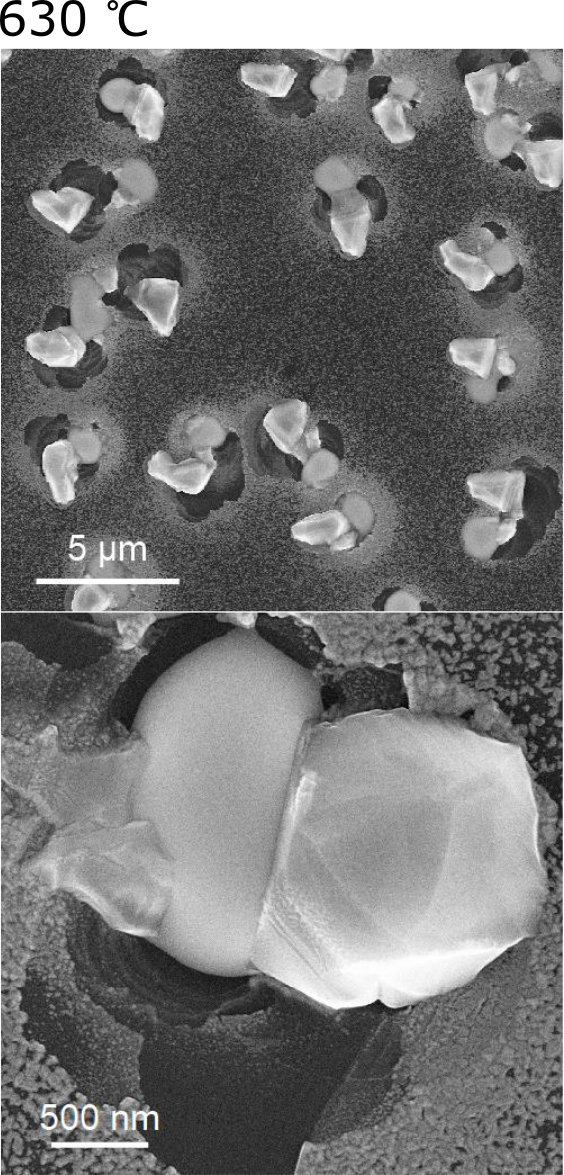
\includegraphics[width=0.25\linewidth]{Image_32_3}} }
				\legend{Температура роста: 550~\si{\degreeCelsius}~(а),
					580~\si{\degreeCelsius}~(б), 630~\si{\degreeCelsius}~(в) (поток As
					4~отн.~ед.)} \caption{РЭМ изображения наноструктур GaAs на Si,
			синтезированных при различных температурах}\label{fig:Image_32}
		\end{figure}

Сравнение РЭМ изображений поверхности образцов указывает на схожесть влияния
повышения температуры и снижения соотношения потоков As/Ga
(см.~рис.~\cref{fig:tab_3} и ~\cref{fig:tab_3_3}): повышение температуры
стимулирует десорбцию As. Это предположение подтверждается накоплением капель
Ga на поверхности при дальнейшем повышении температуры
(см.~рис.~\cref{fig:Image_32_3}).

\begin{figure}[ht] \centerfloat{ \subcaptionbox{\label{fig:tab_3_1}}{%
			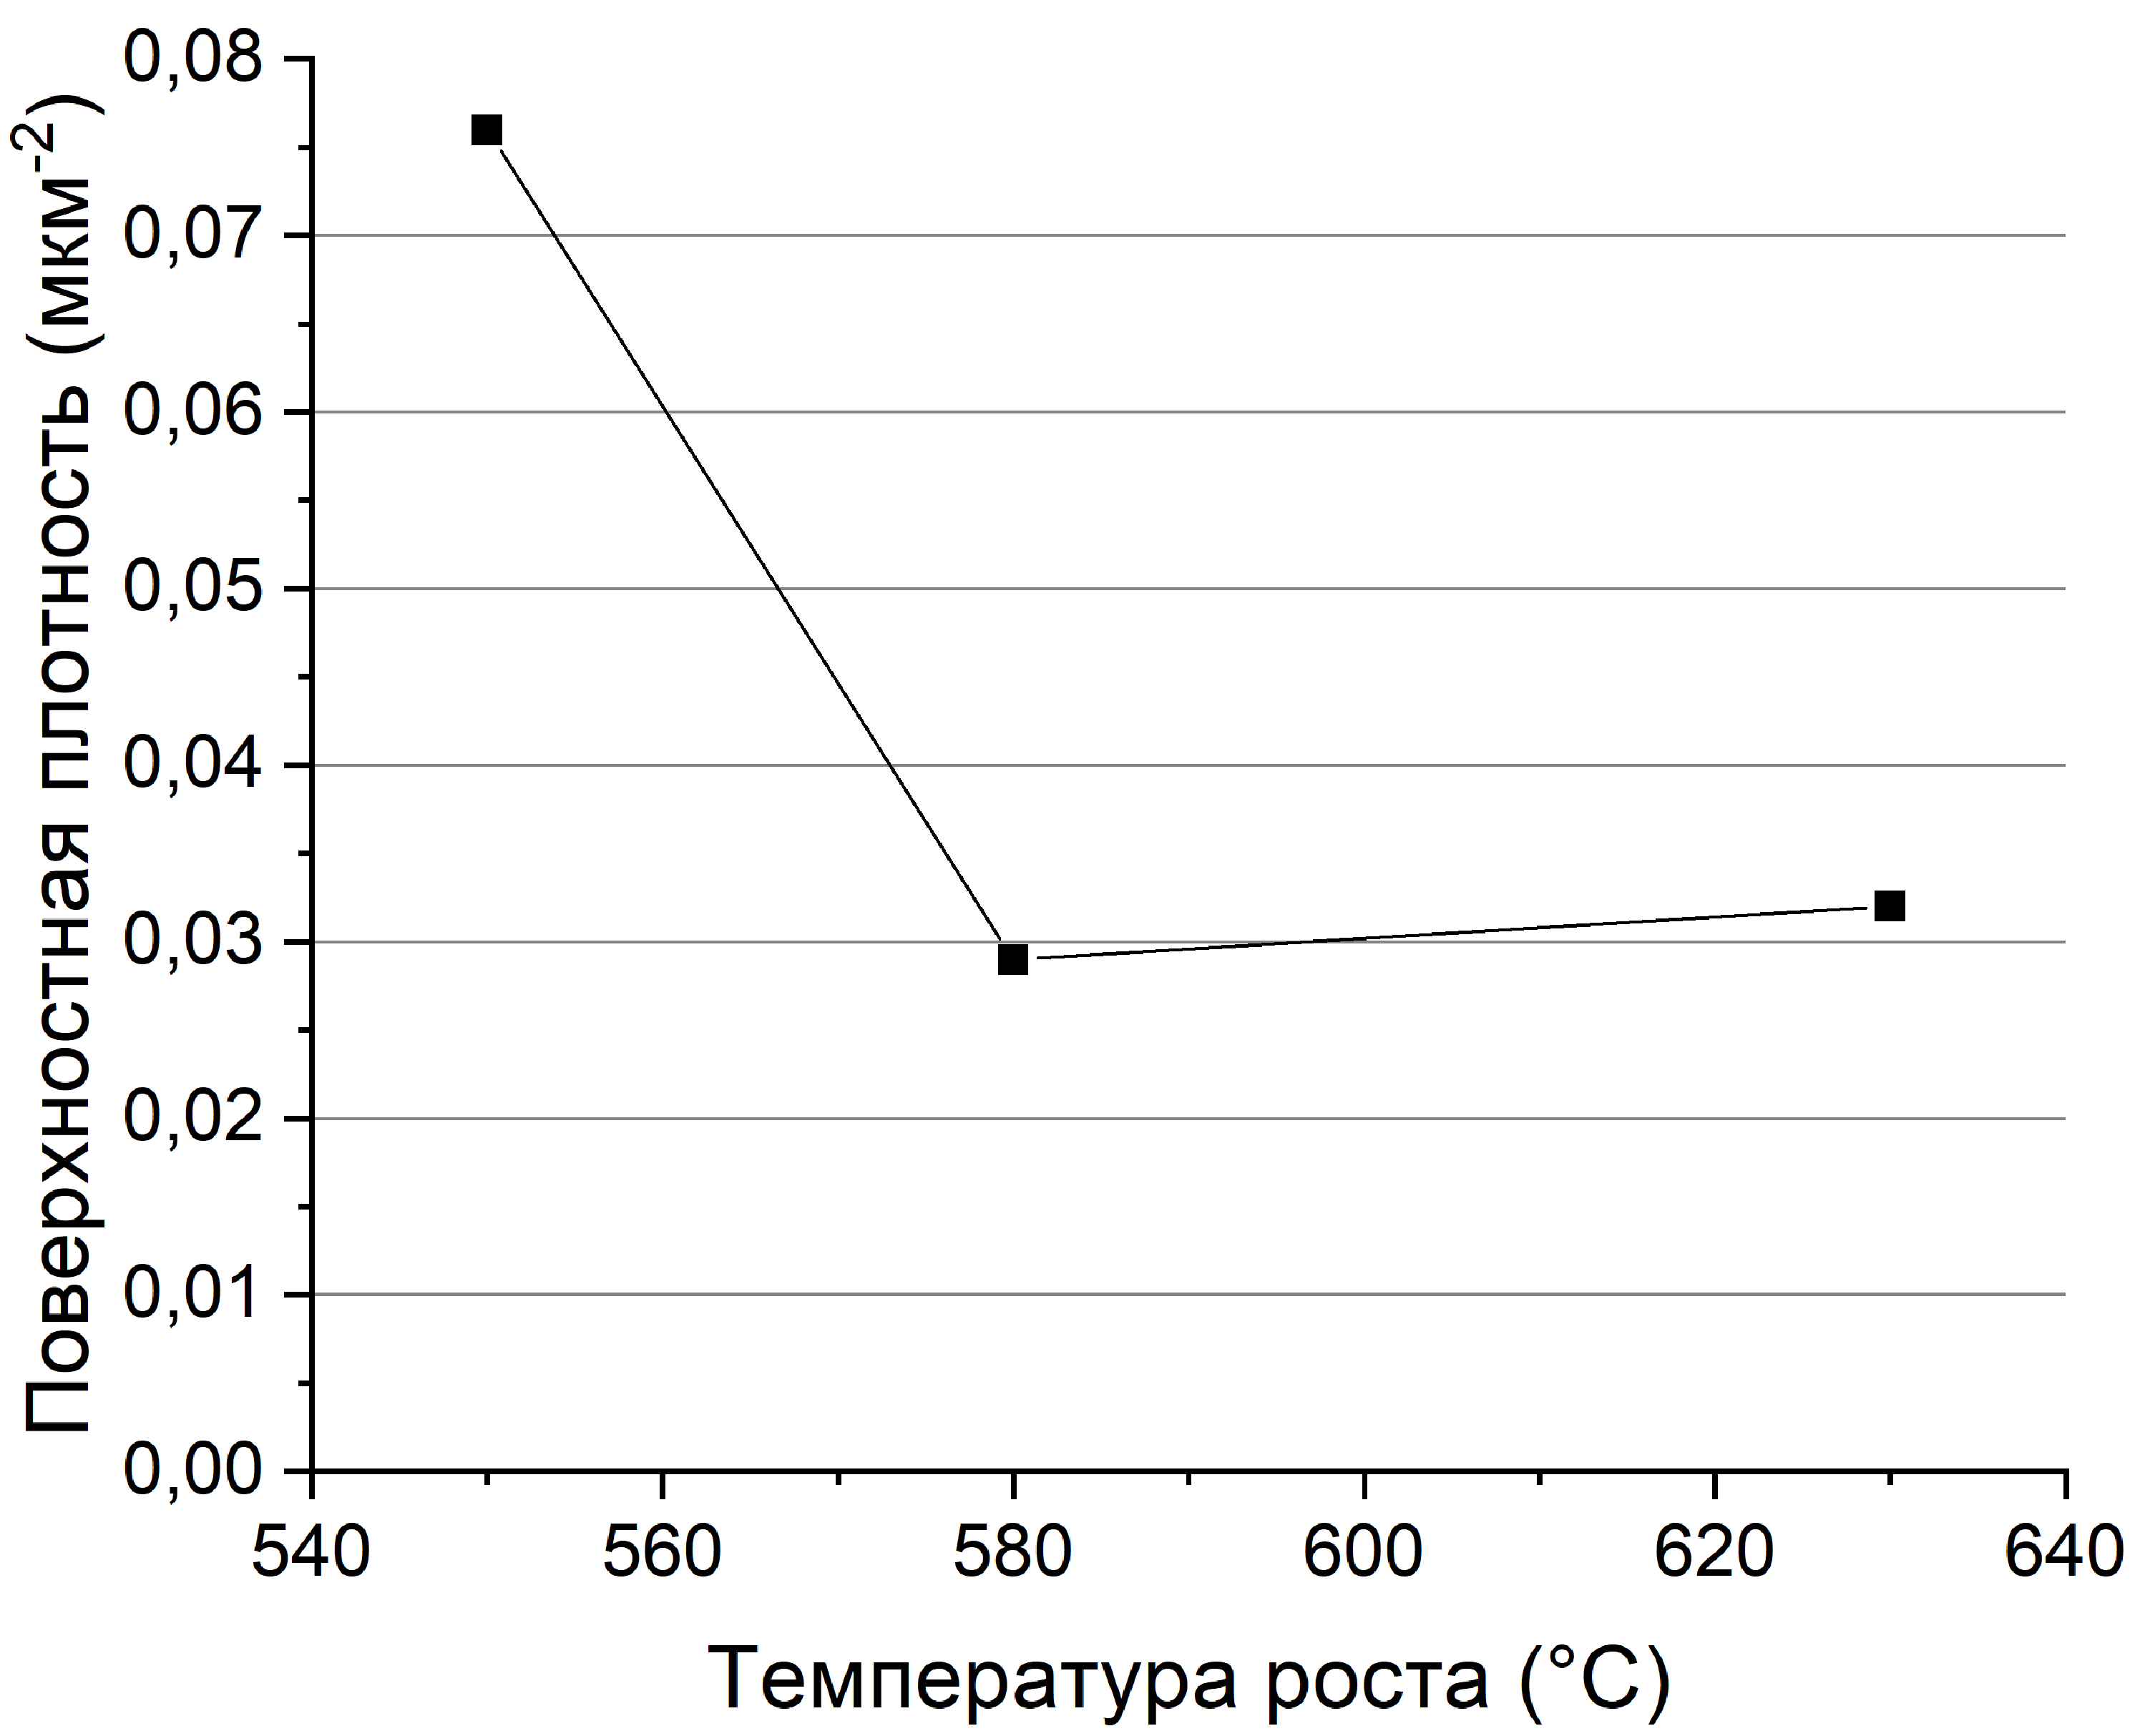
\includegraphics[width=0.48\linewidth]{tab_3_1}}
			\subcaptionbox{\label{fig:tab_3_2}}{%
			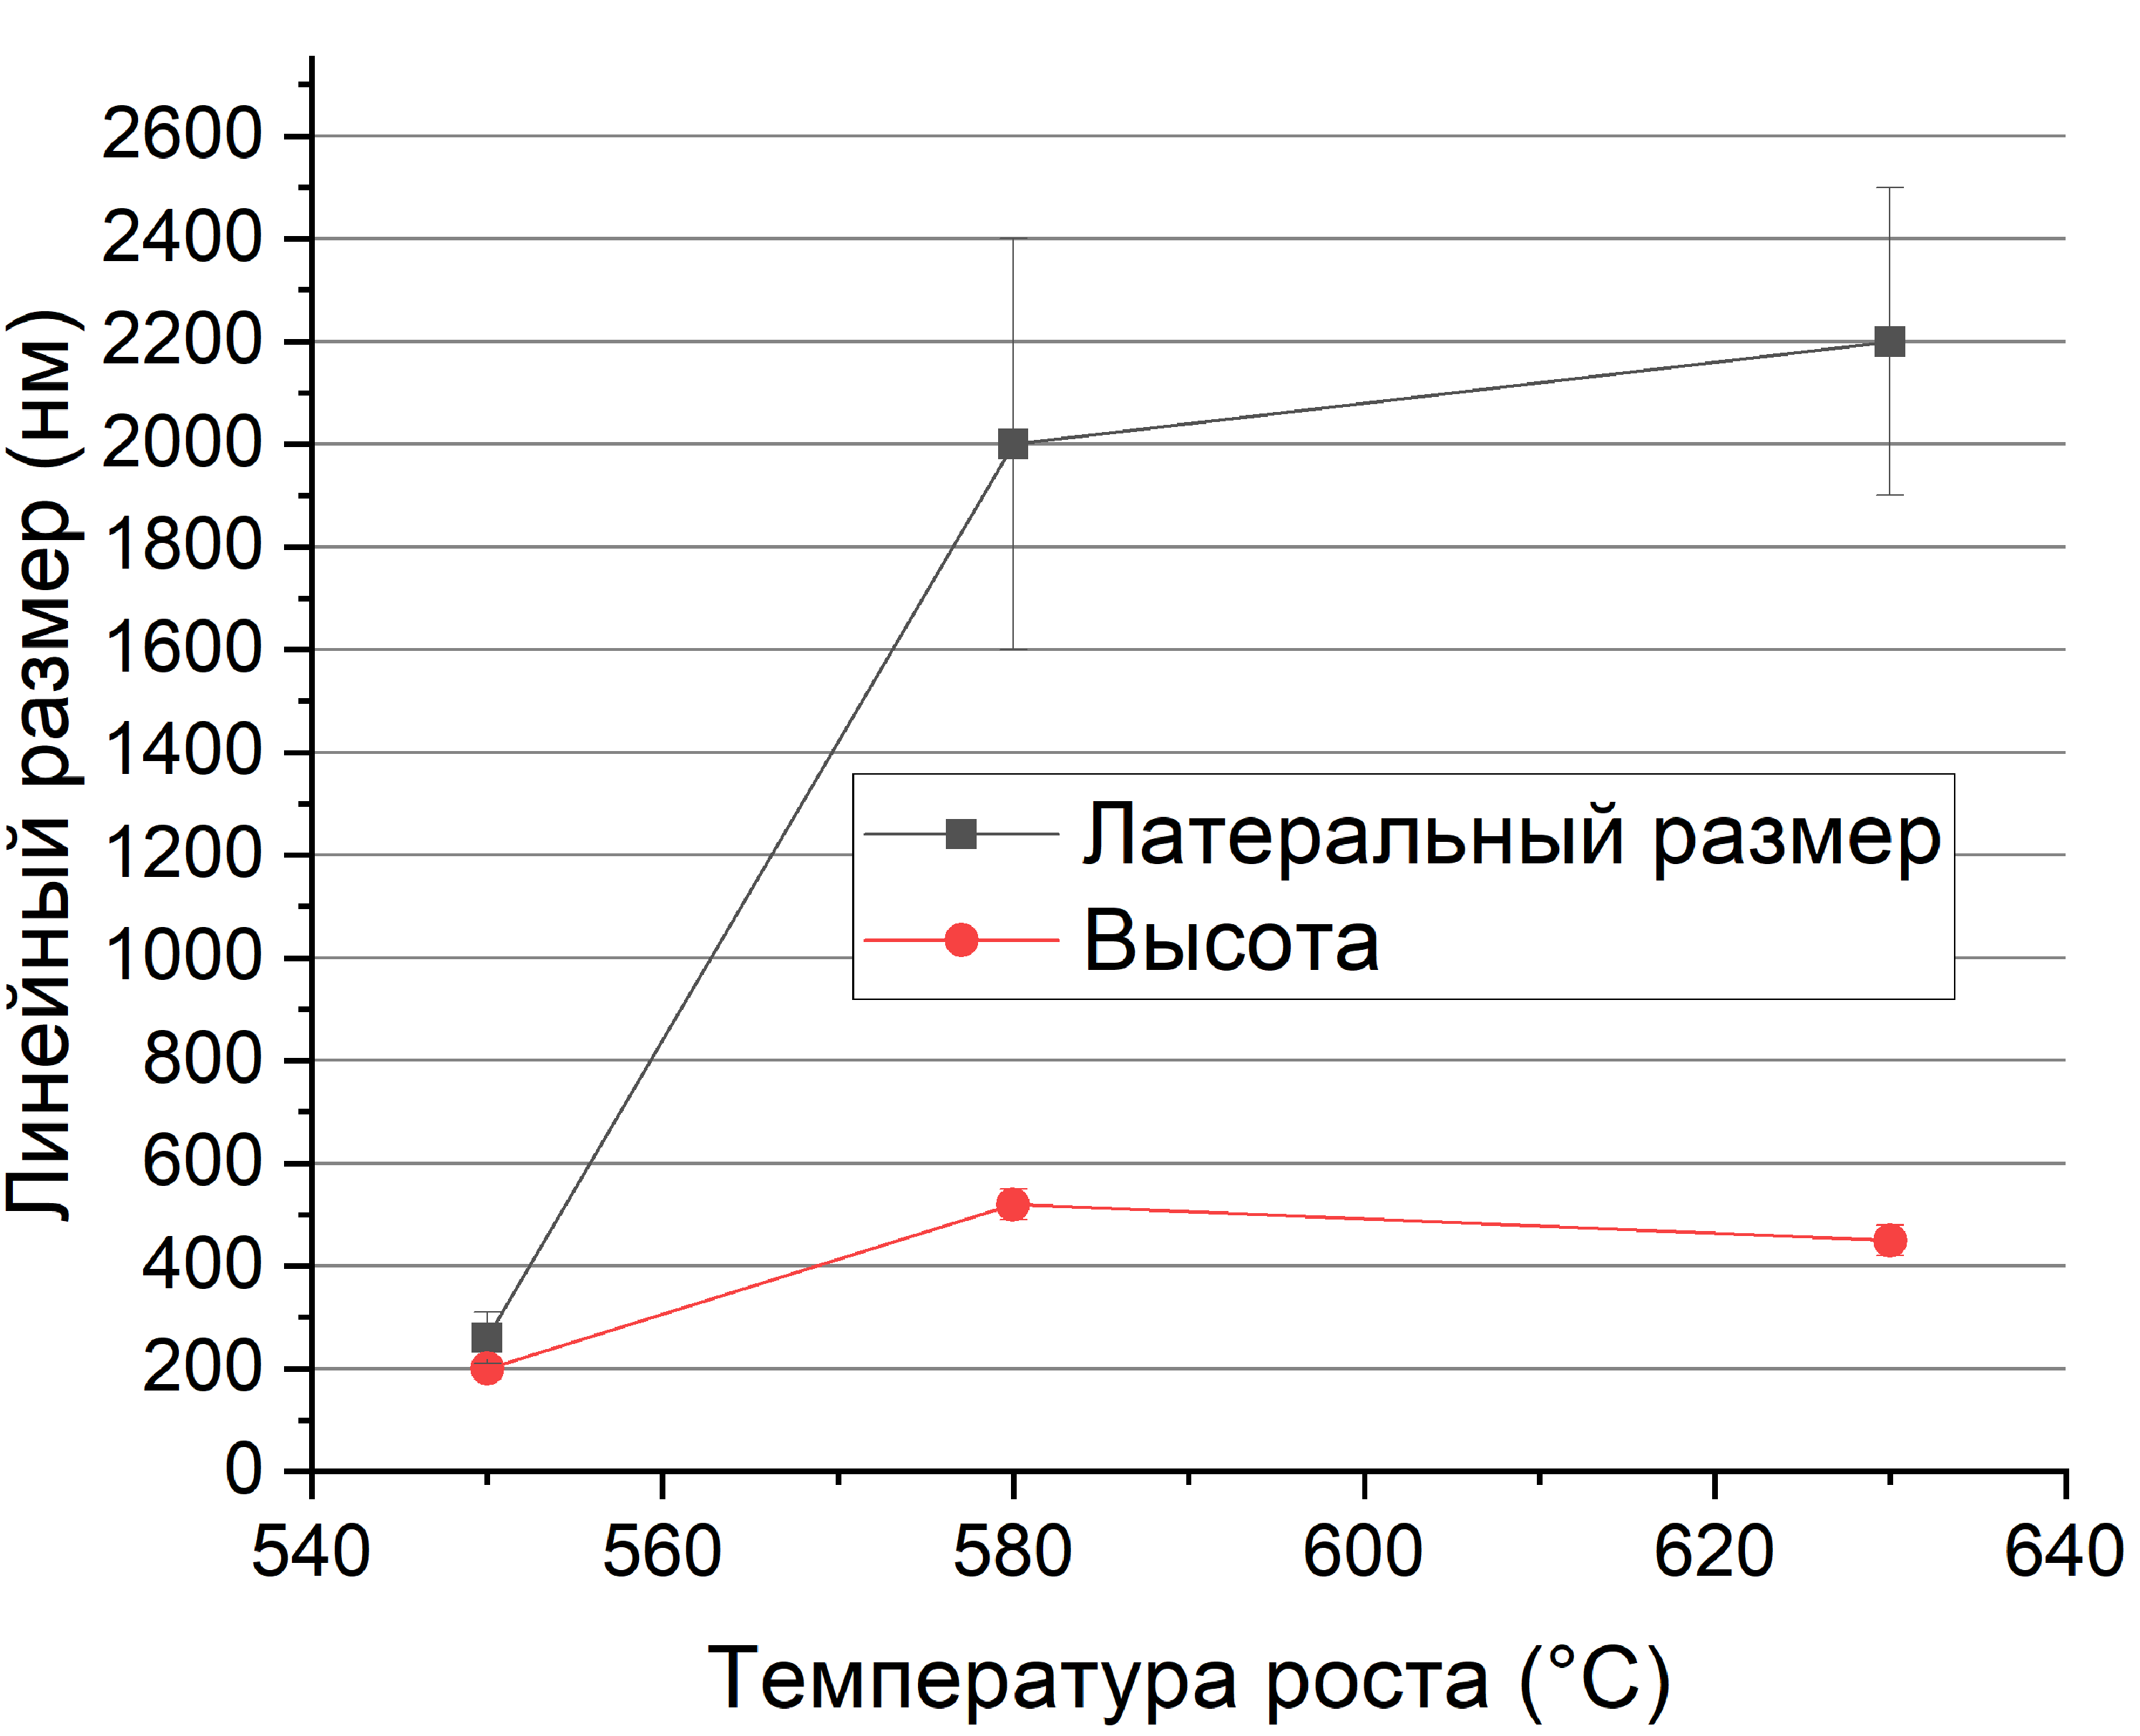
\includegraphics[width=0.48\linewidth]{tab_3_2}} } \legend{Наноструктуры
			GaAs синтезированы при при потоке As в 4~отн.~ед.} \caption{Зависимости
			поверхностной плотности массива~(а) и линейных размеров наночастиц~(б) от
	температуры роста}\label{fig:tab_3} \end{figure}

\begin{figure}[ht] \centerfloat{
		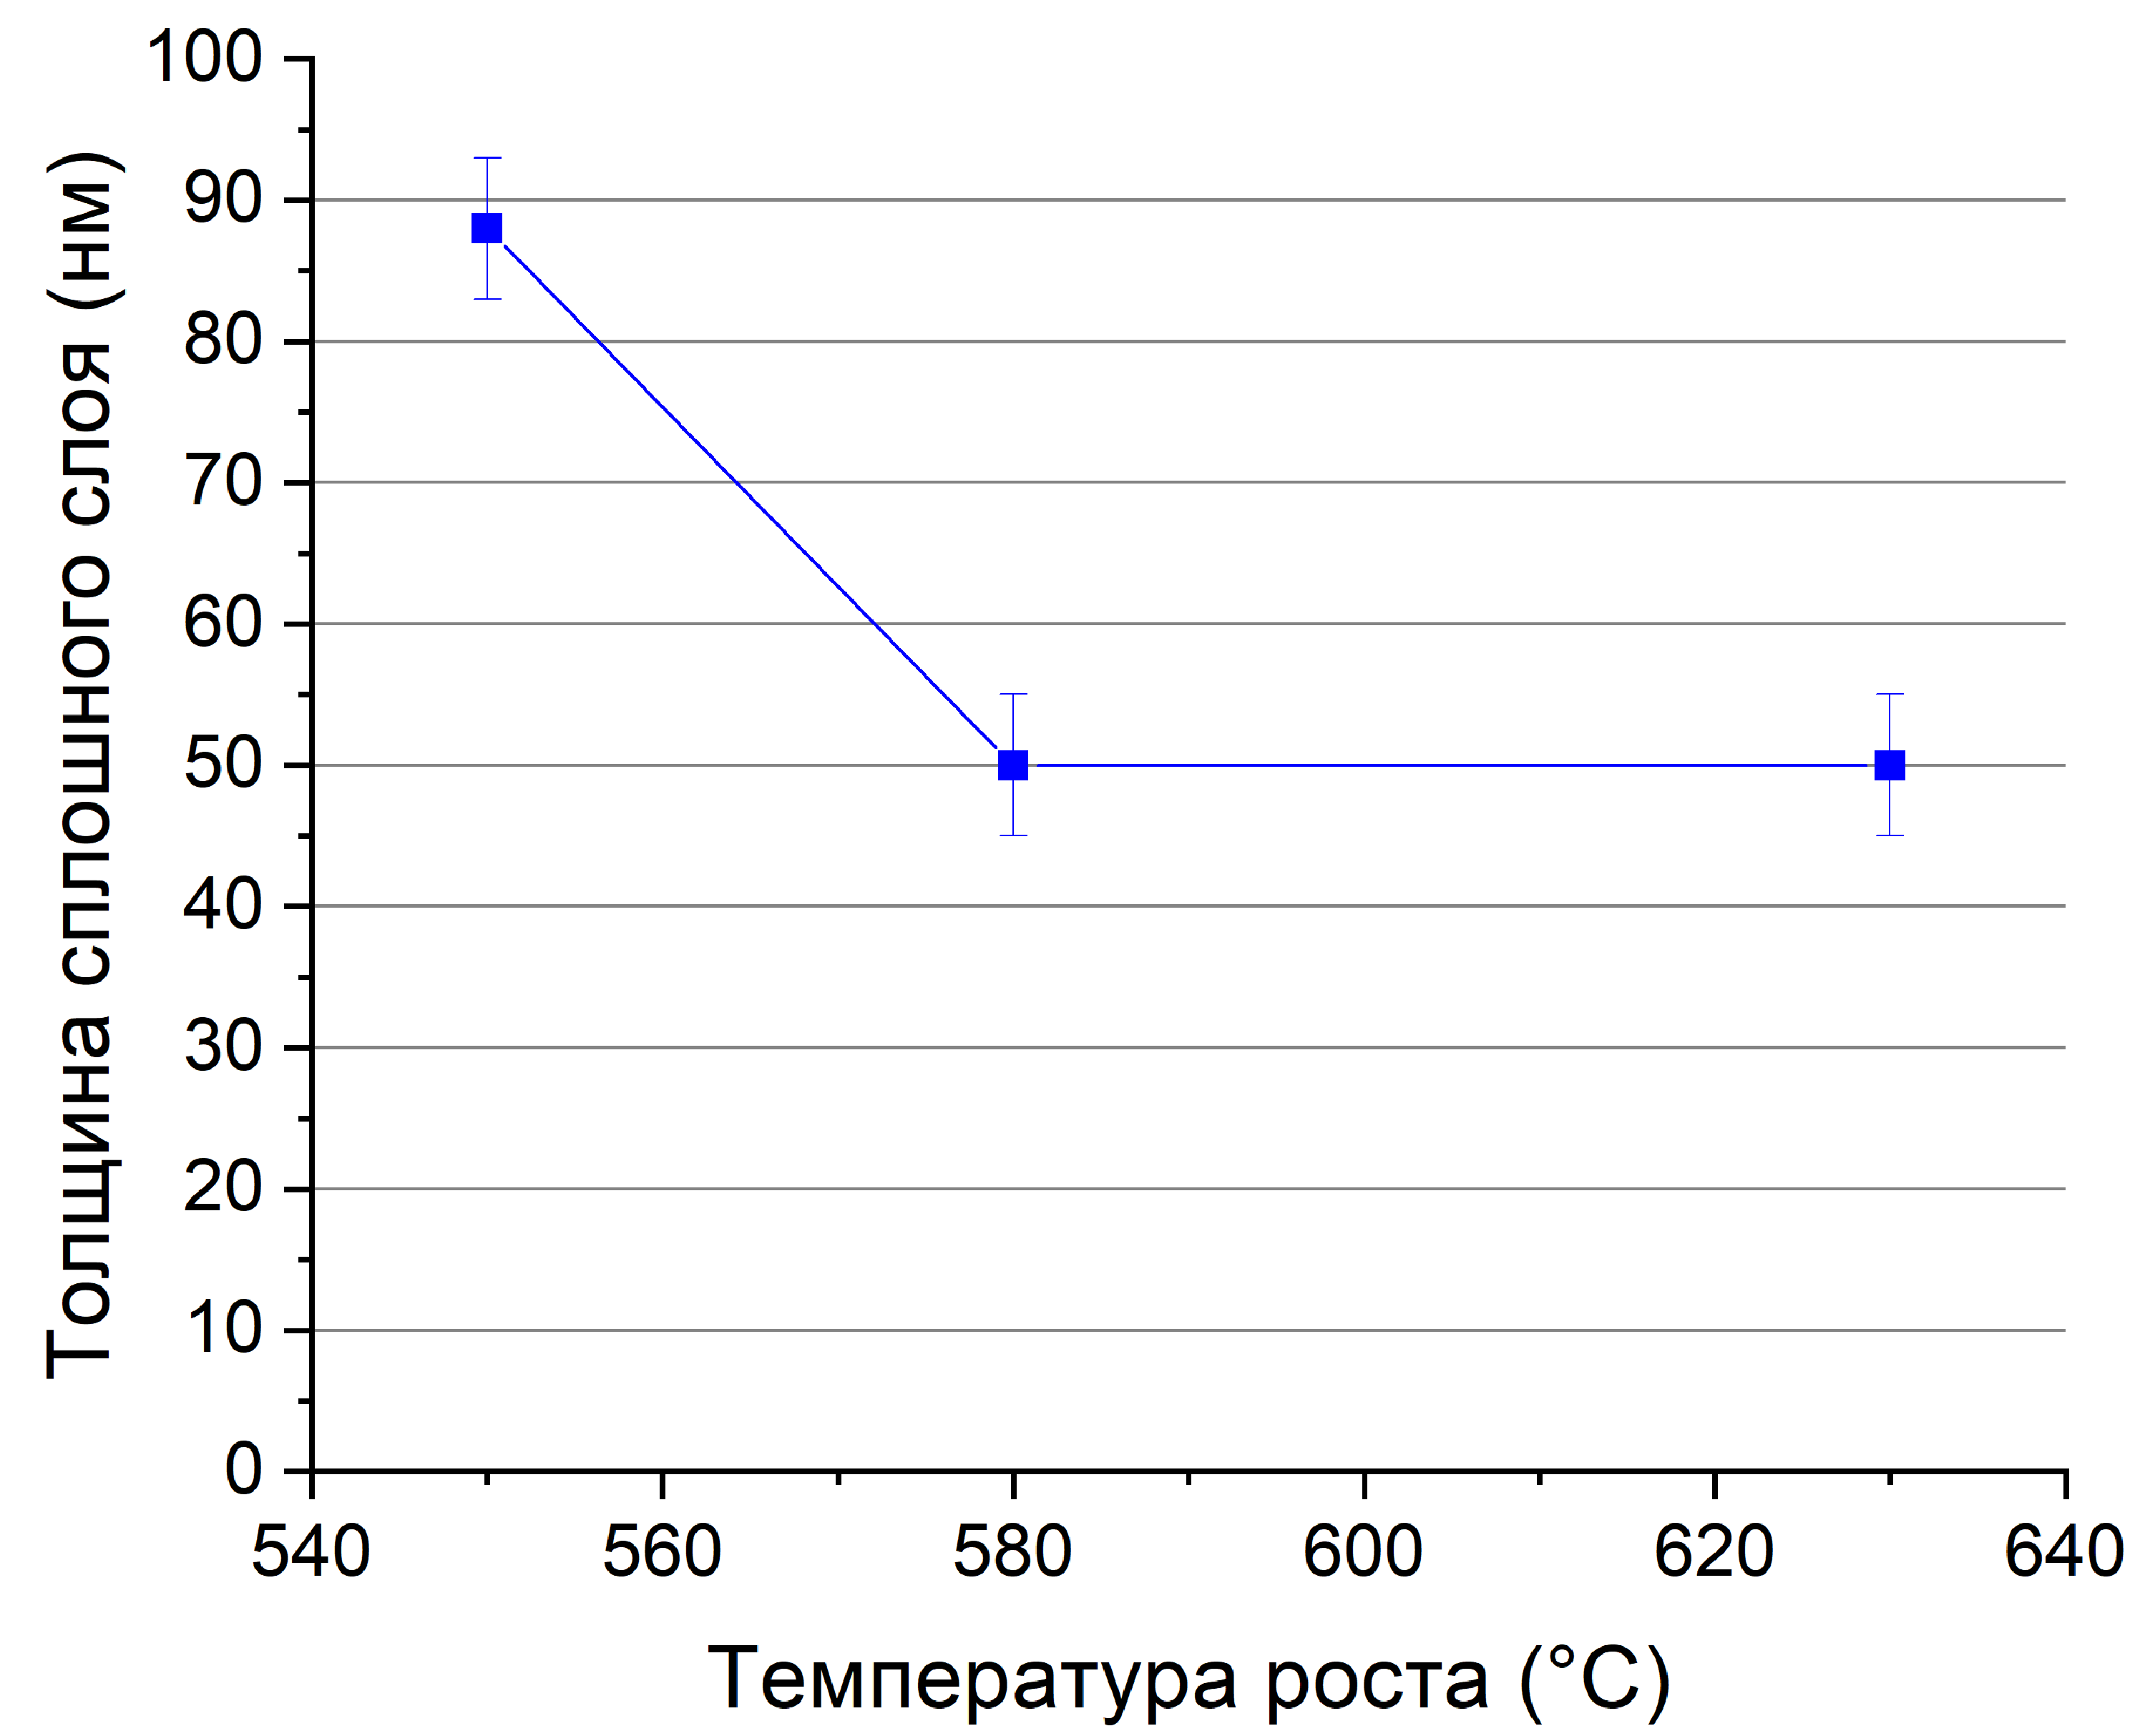
\includegraphics[width=0.48\linewidth]{tab_3_3} } \legend{Наноструктуры
		GaAs синтезированы при при потоке As в 4~отн.~ед.} \caption{Зависимость
		толщины сплошного слоя от температуры роста}\label{fig:tab_3_3}
	\end{figure}

Таким образом, изменение соотношения потоков As/Ga и температуры роста может
использоваться для контроля размеров и плотности наночастиц GaAs.

\subsection{Изменение морфологии в процессе роста}\label{subsec:ch5/sec2/sub2}

Для изучения изменения морфологии наночастиц во время роста выращены два
образца при одинаковых условиях синтеза в течение 10 и 30~\si{\minute}.
Температура роста образцов~--- 550°C, поток As в 4~отн.~ед. Площадь области
свободной от кристаллизованного GaAs, окружающей наночастицы, и поверхностная
плотность наночастиц значительно уменьшается (с 0,08 до
0,007~\si{\per\micro\metre\squared}) во время роста
(см.~рис.~\cref{fig:Image_33}).

\begin{figure}[ht] \centerfloat{ \subcaptionbox{\label{fig:Image_33_1}}{%
			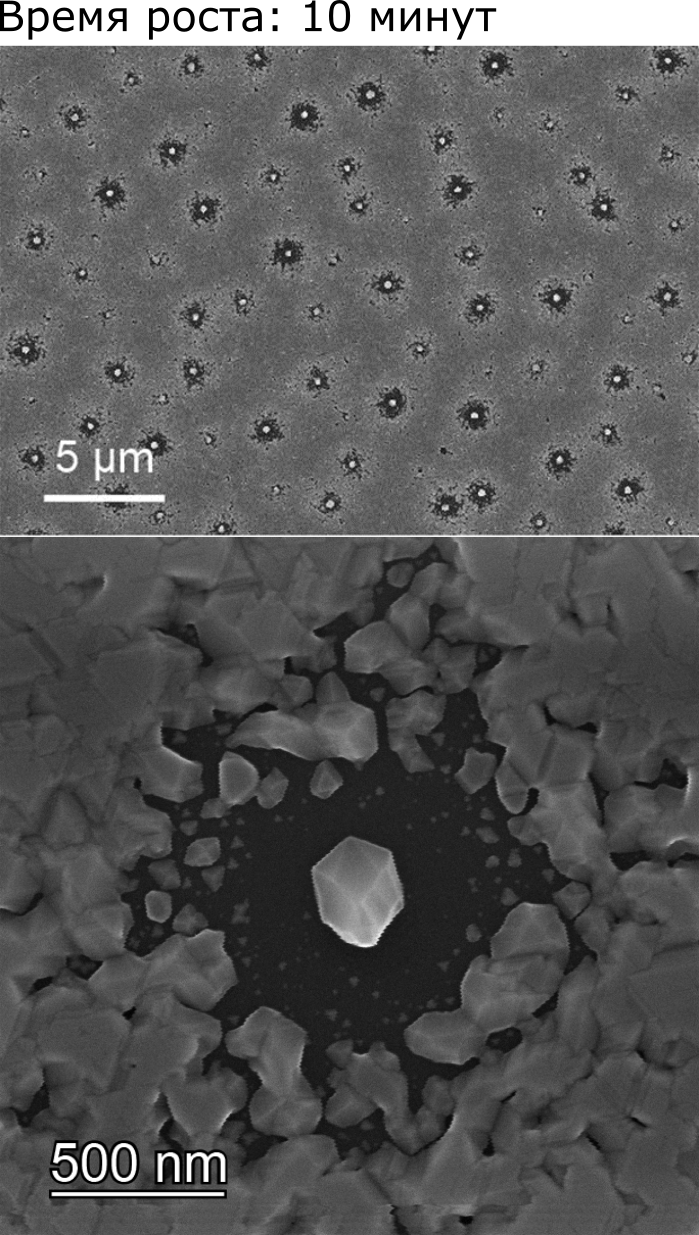
\includegraphics[width=0.4\linewidth]{Image_33_1}}
			\subcaptionbox{\label{fig:Image_33_2}}{%
			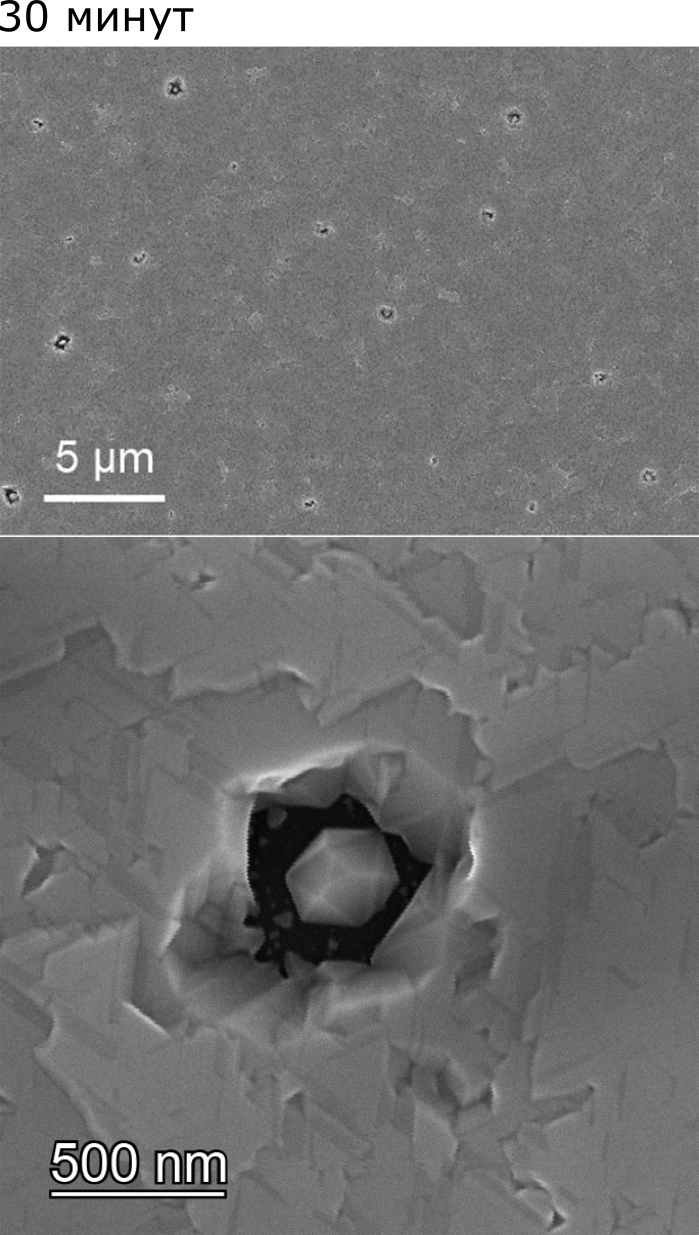
\includegraphics[width=0.4\linewidth]{Image_33_2}} } \legend{Температура
			роста образцов 550~\si{\degreeCelsius}, поток As в 4~отн.~ед.}
			\caption{РЭМ изображения эпитаксиальных наночастиц GaAs на поверхности
				Si, выращенных в течение 10~(а) и
		30~\si{\minute}~(б)}\label{fig:Image_33} \end{figure}

Сплошной слой образован слиянием наноостровков (см.~рис.~\cref{fig:Image_33},
\cref{fig:Image_34}) с гранями, параллельными поверхности подложки
(111)\textsubscript{Si}. Высота и латеральный размер наночастиц, выращенных в
течении 30~\si{\minute}, остаётся близкой к высоте наночастиц, синтезированных
в течение 10~\si{\minute}. При этом толщина сплошного слоя увеличилась с
\(\approx 50\) до \(\approx 200\)~\si{\nano\metre}
(см.~рис.~\cref{fig:Image_34}).

\begin{figure}[ht] \centerfloat{ \subcaptionbox{\label{fig:Image_34_1}}{%
			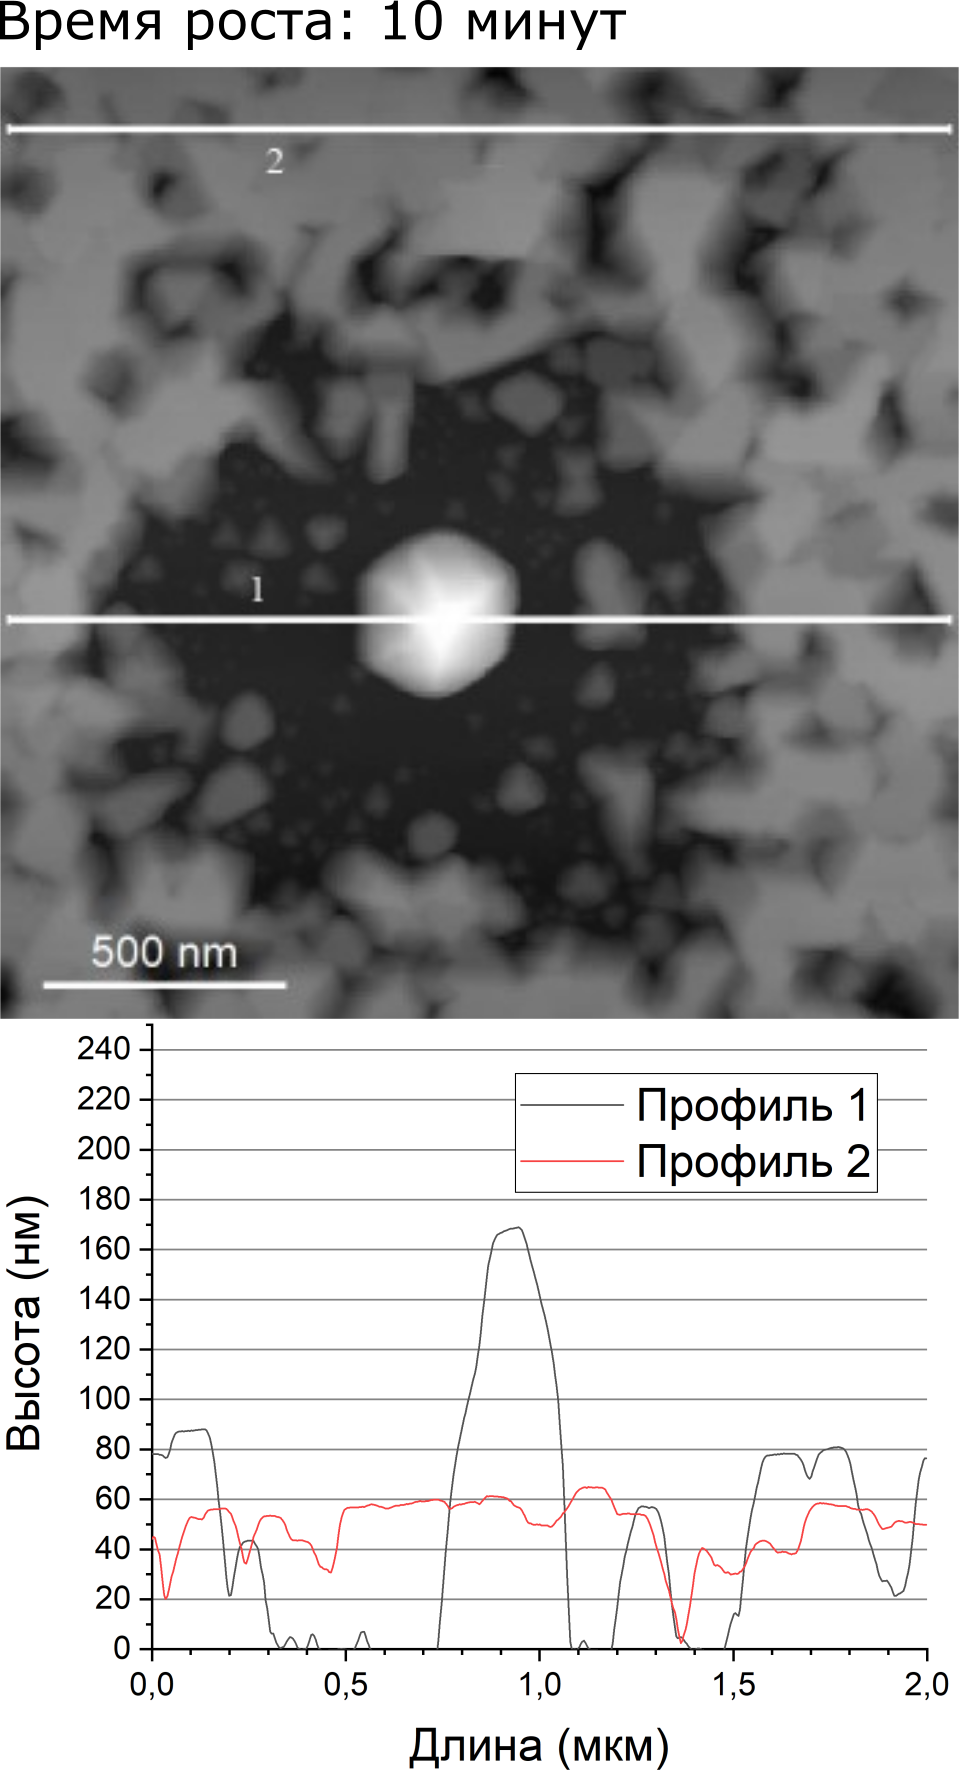
\includegraphics[width=0.4\linewidth]{Image_34_1}}
			\subcaptionbox{\label{fig:Image_34_2}}{%
			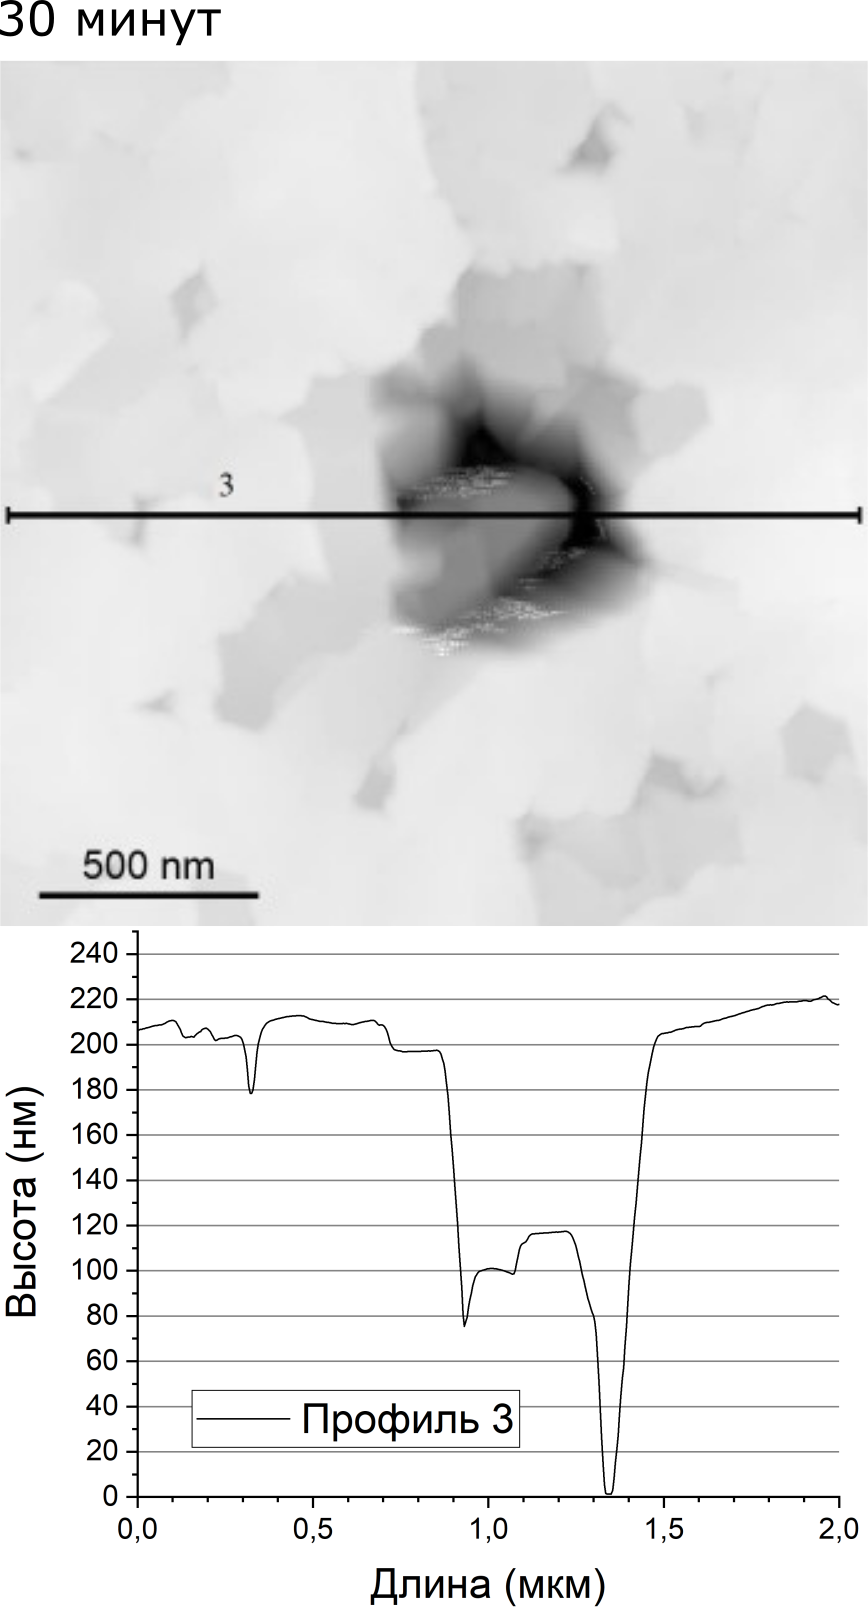
\includegraphics[width=0.4\linewidth]{Image_34_2}} } \legend{Температура
			роста образцов 550~\si{\degreeCelsius}, поток As в 4~отн.~ед. Линии на
			изображениях АСМ соответствуют профилям высот} \caption{АСМ изображения и
			профили высот эпитаксиальных наночастиц GaAs на поверхности Si,
			выращенных в течение 10 (а) и 30~\si{\minute} (б)}\label{fig:Image_34}
		\end{figure}

Зарастание сплошным слоем в процессе роста косвенно подтверждает предположение,
что наночастицы GaAs образуются по механизму ПЖК. Можно предположить, что
скорость их роста значительно уменьшается после кристаллизации капли, поскольку
поступающий материал начинает преимущественно встраиваться в сплошной слой.

Эквивалентная толщина выращенного за 30 минут материала составляет \(\approx
200\)~\si{\nano\metre}, что соответствует скорости роста
0,4~\si{\micro\metre\per\hour}. Эта скорость роста соответствует скорости
гомоэпитаксии планарного GaAs/GaAs(001) при том же потоке Ga и температуре
роста.

На трёхмерном АСМ изображении выращенной в течение 10~\si{\minute} наночастицы
можно различить огранку (см.~рис.~\cref{fig:Image_35_2}). Двумерный график
функции распределения наклонов в полярных координатах представлен
на~рис.~\cref{fig:Image_35_3}. Центральная особенность соответствует непокрытой
поверхности подложки и верхней грани наночастицы. Учитывая эпитаксиальную
ориентацию наночастиц, можно сделать вывод, что верхняя грань имеет ту же
ориентацию, что и поверхность подложки – ориентацию \{111\}.

\begin{figure}[ht] \centerfloat{ \subcaptionbox{\label{fig:Image_35_1}}{%
			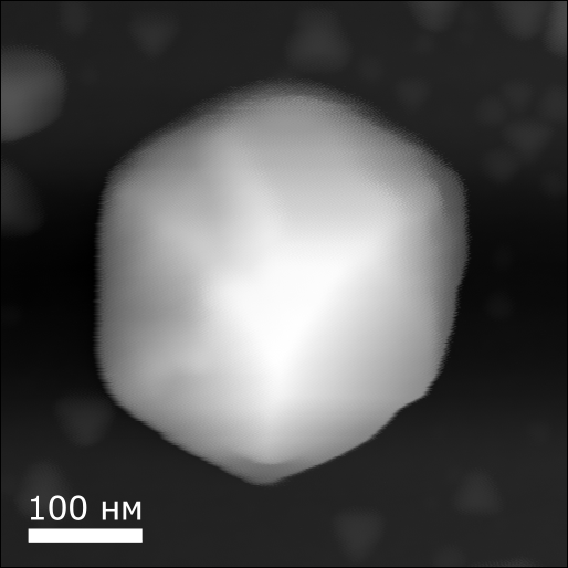
\includegraphics[height=5cm]{Image_35_1}}
			\subcaptionbox{\label{fig:Image_35_2}}{%
			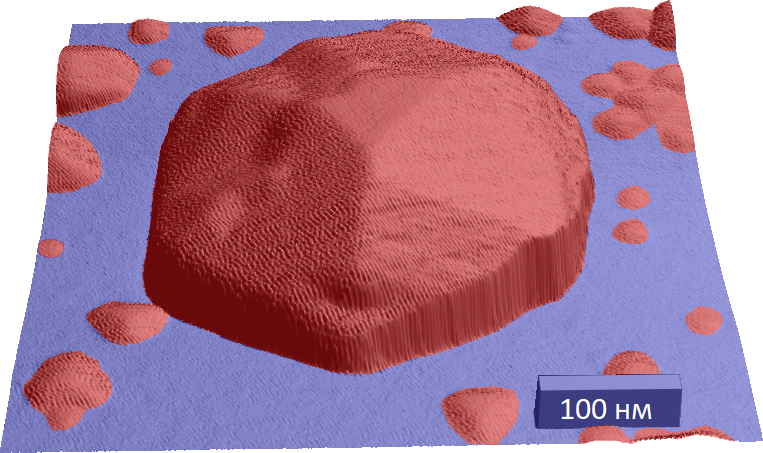
\includegraphics[height=5cm]{Image_35_2}}

		\subcaptionbox{\label{fig:Image_35_3}}{%
		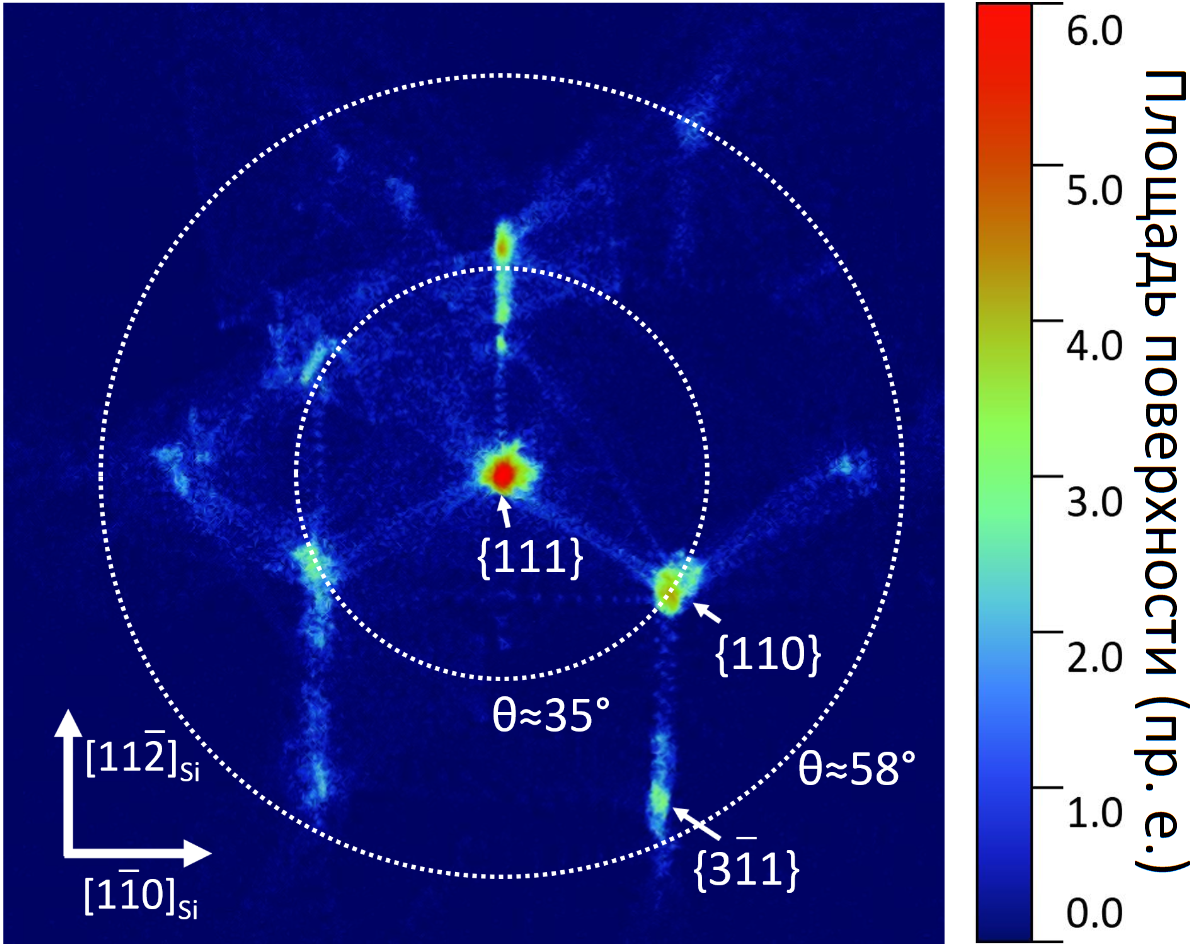
\includegraphics[width=0.65\linewidth]{Image_35_3}} } \legend{На
		графике~(в) радиальное расстояние от центра соответствует углу наклона
		граней относительно нормали подложки, а угол \(\phi\) соответствует
		азимутальной ориентации грани.  Интенсивность особенности соответствует
		общей площади поверхности, имеющей соответствующий наклон
		(\(\phi\),~\(\theta\)). Круги соответствуют наклону грани \(\theta =
		35\){\textdegree} и \(\theta = 58\){\textdegree}} \caption{АСМ изображение
		наночастицы GaAs~(а), её трехмерное изображение~(б) и график функции
		распределения наклона в полярных координатах
S(\(\theta\)(r),~\(\phi\))~(в)}\label{fig:Image_35} \end{figure}

Радиальное расстояние от центра на графике функции распределения наклонов
соответствует углу \(\theta\) наклона граней относительно нормали подложки.
Угол \(\phi\) соответствует азимутальной ориентации грани. Интенсивность
особенности на графике функции распределения наклонов соответствует общей
площади поверхности, имеющей соответствующий наклон (\(\phi\),~\(\theta\)).

На графике функции распределения наклонов можно выделить два набора
особенностей с наклоном граней \(\theta\approx 35\){\textdegree} и
\(\theta\approx 58\){\textdegree}. Три грани с наклоном \(\theta\approx 35 \pm
5\){\textdegree} можно отнести к плоскостям \{110\}, поскольку угол между (111)
и (110) равен 35,26{\textdegree}. Эти грани азимутально (\(\phi\)) выровнены
вдоль направлений <\(11\overline{2}\)>\textsubscript{Si}, соответствующих
проекциям направлений <110> на плоскость (111). Азимутальный угол (\(\phi\))
между этими гранями близок к 120{\textdegree}, что указывает на трёхкратную
симметрию кристаллической решётки ZB вдоль направления [111].

Шесть других особенностей на графике функции распределения наклонов с
\(\theta\approx 52 \pm 3\){\textdegree}, можно отнести к характерным для
огранки GaAs плоскостям \{\(3\overline{1}1\)\} \cite{Yeu2019, wong2010},
поскольку угол между (111) и \{\(3\overline{1}1\)\} равен 58,52{\textdegree}.
Эти грани азимутально (\(\phi\)) расположены через каждые 60{\textdegree} и
смещены на \(28 \pm 7\){\textdegree} относительно граней \{110\}, что хорошо
согласуется с азимутальной ориентацией (\(\phi\)) между гранями
\{\(3\overline{1}1\)\} и \{110\} (см.~рис.~\cref{fig:Image_35_3}).

На поверхности образца имеются наночастицы с двойникованием, у которых набор
граней развернут на 180{\textdegree} вокруг нормали к подложке. Вращательное
двойникование также наблюдалось на картине ДБЭ вдоль направления
[\(1\overline{1}0\)]\textsubscript{Si} с дифракционными рефлексами двойниковой
ZB структуры GaAs.

Образование грани GaAs (111)A энергетически более выгодно, чем образование
(111)B грани \cite{Tomioka2009, wong2010}. Удельная площадь (111) граней
сросшихся островков сплошного слоя выше аналогичной площади у наночастиц
(см.~рис.~\cref{fig:Image_33}, \cref{fig:Image_34}). Из этого можно сделать
вывод, что сросшиеся островки сплошного слоя и наночастицы имеют A и B
полярность соответственно (см.~подраздел~\cref{subsec:ch1/sec2/sub4}).

Наночастица на~рис.~\cref{fig:Image_34_2} заросла сплошным слоем, но сохранила
различимые грани \{\(3\overline{1}1\)\} и \{110\}. Можно предположить, что эти
грани становятся границами инверсионного домена после слияния наночастиц и
сплошного слоя с противоположной полярностью в процессе роста.

\subsection{Исследование КРС и ФЛ от наночастиц}\label{subsec:ch5/sec2/sub3}

Карта пространственной зависимости интегральной интенсивности в области
поперечного оптического (TO) фононного пика GaAs со структурой ZB представлена
на~рисунке~\cref{fig:Image_36_1}. Спектры измерялись при комнатной температуре,
плотности мощности лазерного возбуждения \(\approx 6 \cdot
10^4\)~\si{\watt\per\centi\metre\squared}, диаметр лазерного пятна \(\approx
6\)~\si{\micro\metre} (мощность лазера \(\approx 0,46\)~\si{\milli\watt}).
Яркий сигнал от наночастиц виден в центре тёмных круглых областей подложки Si
без синтезированного материала.

\begin{figure}[ht] \centerfloat{ \subcaptionbox{\label{fig:Image_36_1}}{%
			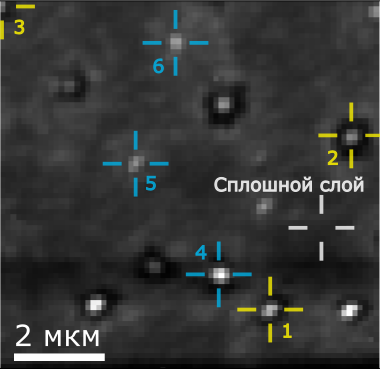
\includegraphics[height=5cm]{Image_36_1}}
			\subcaptionbox{\label{fig:Image_36_2}}{%
			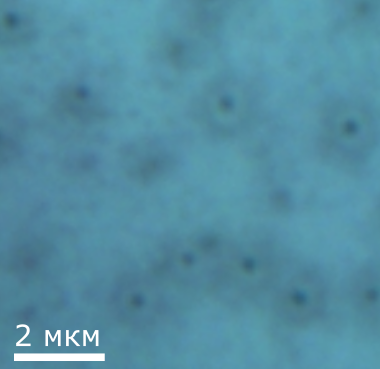
\includegraphics[height=5cm]{Image_36_2}}

		\subcaptionbox{\label{fig:Image_36_3}}{%
		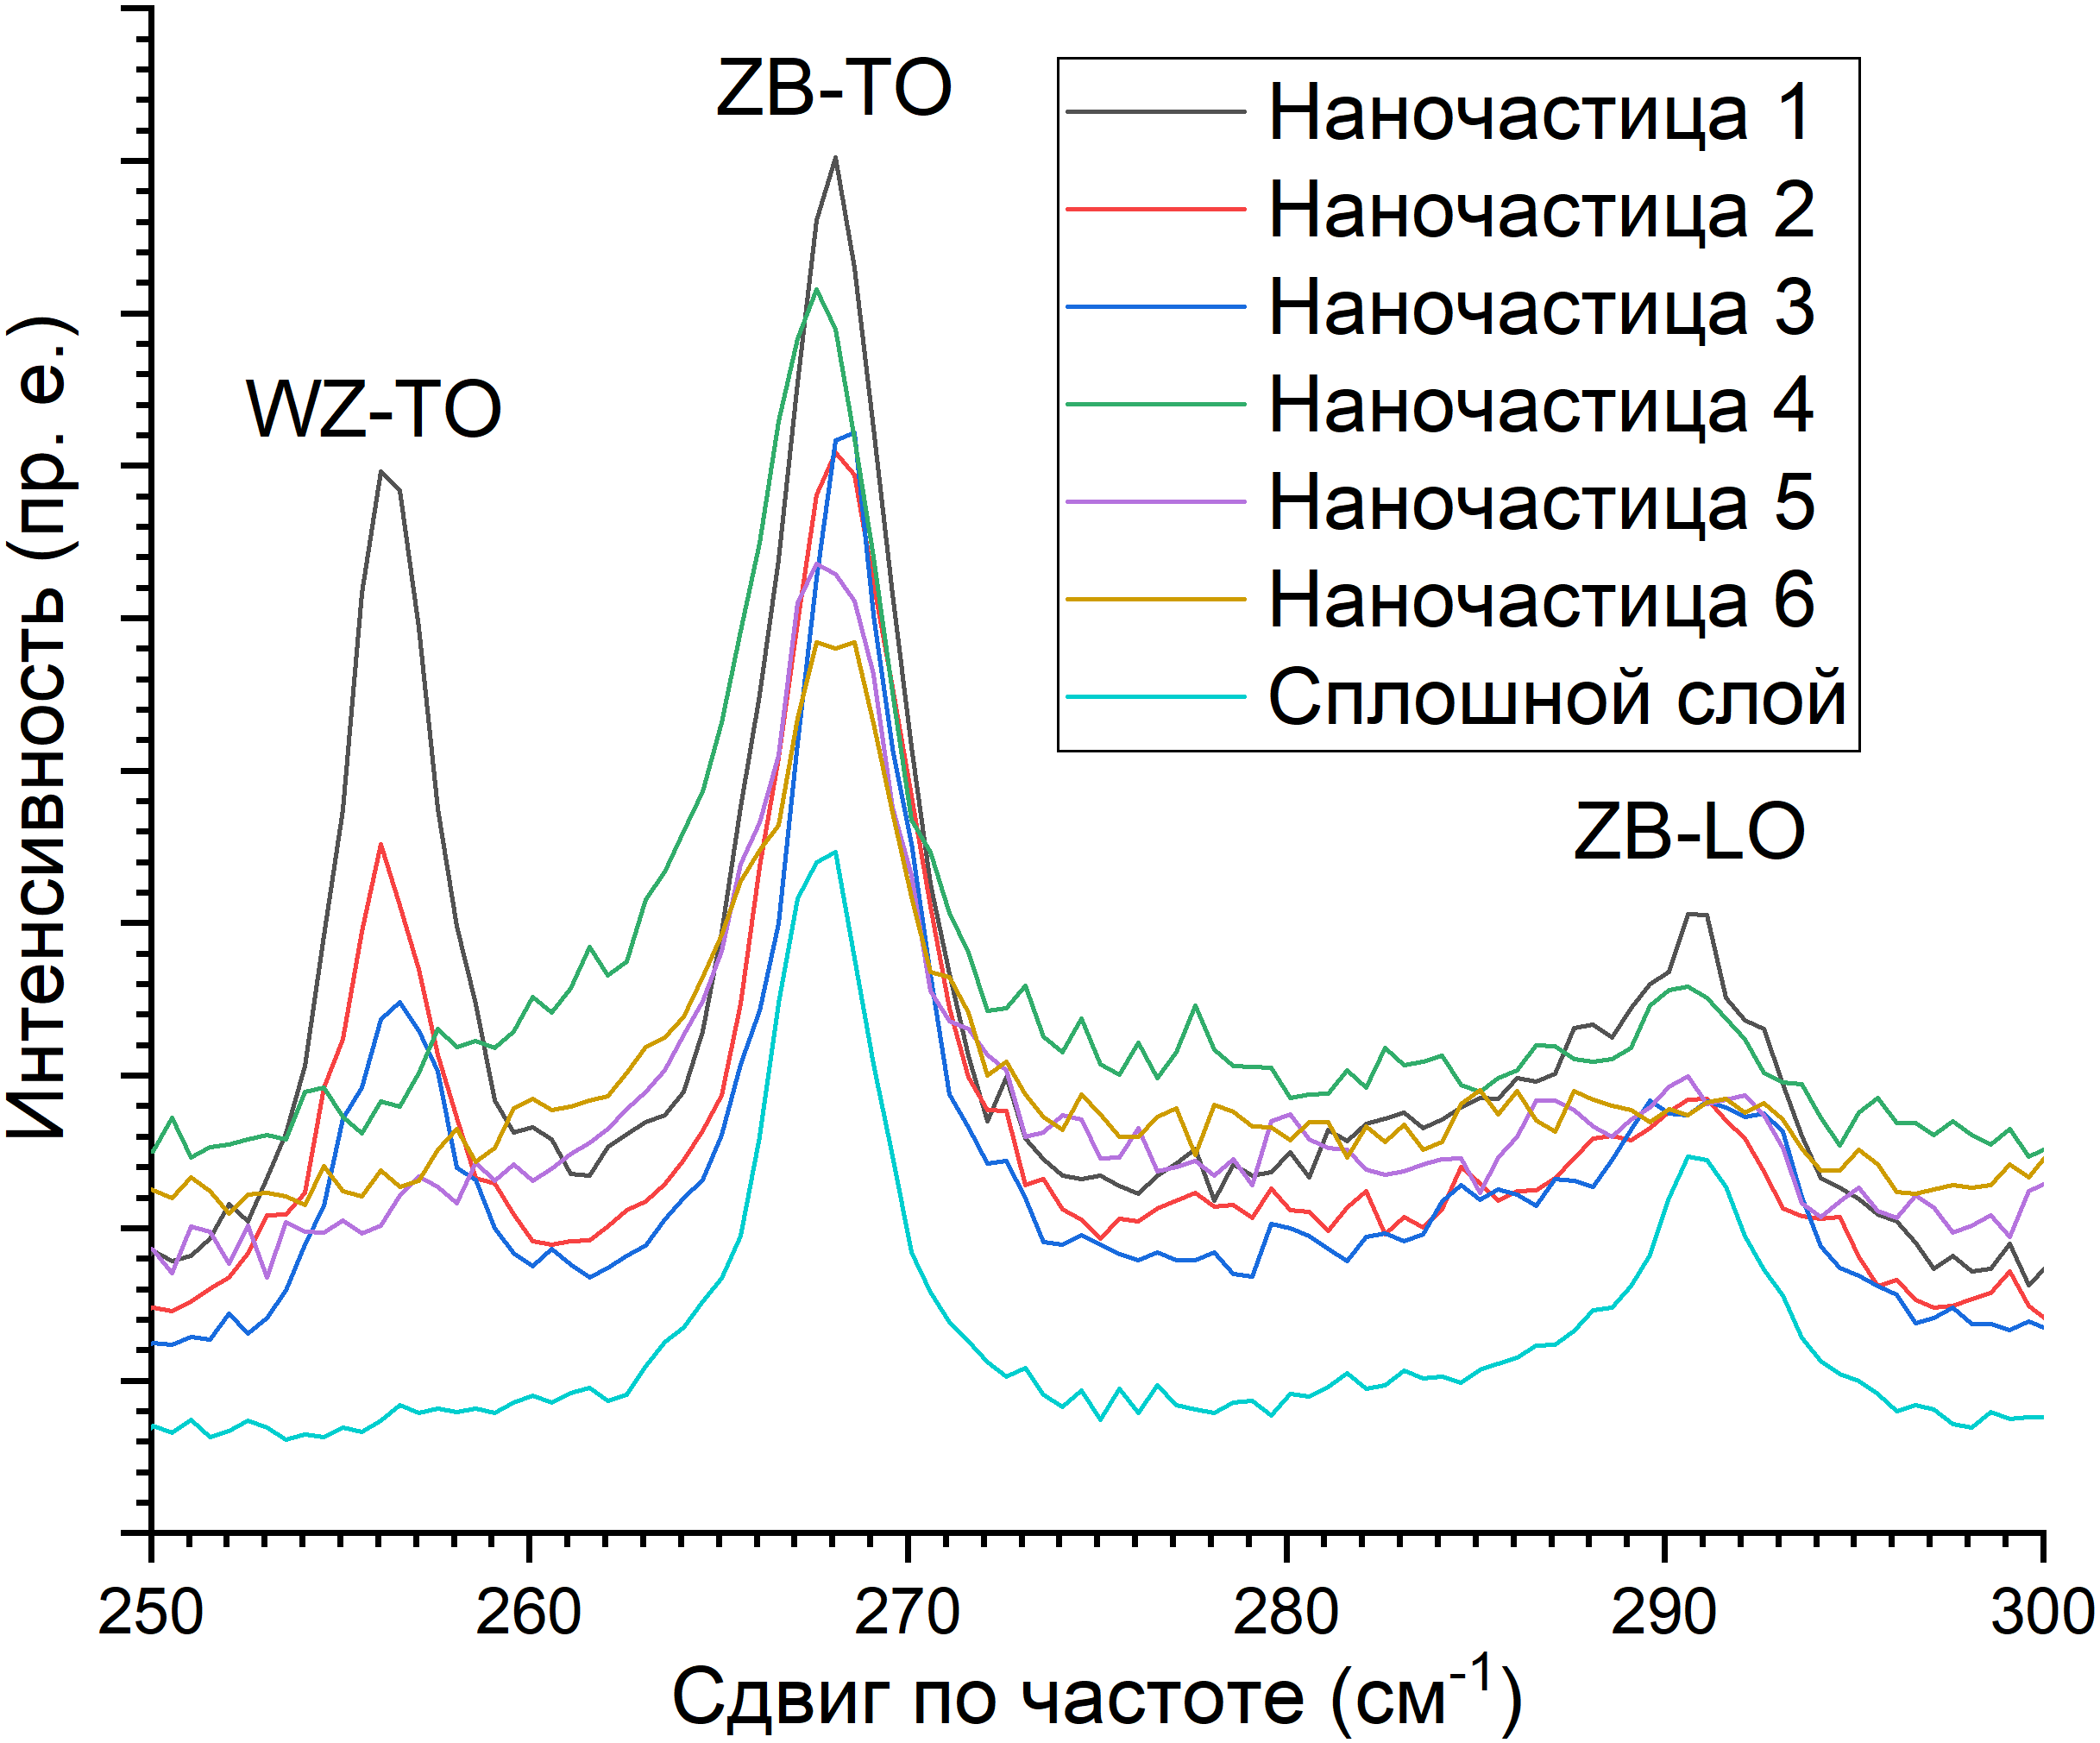
\includegraphics[width=0.7\linewidth]{Image_36_3}} } \legend{Наночастицы,
		КР спектры которых имеют WZ пик на 256~\si{\per\centi\metre}, отмечены
		жёлтыми маркерами (1--3). КР спектры остальных наночастиц, включая те, что
		отмечены синими маркерами (4--6), имеют только ZB фононные моды}
		\caption{Карта пространственной зависимости интегральной интенсивности
			ZB-TO моды, снятая при комнатной температуре от образца, выращенного при
			550~\si{\degreeCelsius} и потоке As в 4~ед. (а). Оптическое изображение
	исследуемой области (б). Спектры КР, снятые в отмеченных точках
	(в)}\label{fig:Image_36} \end{figure}

Спектры КР в диапазоне 250--300~\si{\per\centi\metre} от отмеченных
на~рисунке~\cref{fig:Image_36_1} областей показаны
на~рисунке~\cref{fig:Image_36_3}. Поперечная оптическая мода ZB GaAs (ZB-TO) на
268~\si{\per\centi\metre} и продольная оптическая мода ZB GaAs (ZB-LO) на
292~\si{\per\centi\metre} различимы на спектрах КРС от сплошного слоя и всех
наночастиц \cite{Signorello2014}.

GaAs и Si имеют несоответствие кристаллографических решёток 4,2\%, но на
спектрах КРС от наночастиц и сплошного слоя не наблюдается сдвиг энергии
фононных TO и LO мод GaAs, что указывает на релаксацию напряжений в
наноструктурах GaAs \cite{Alekseev2017}.

На спектрах наночастиц GaAs, отмеченных жёлтыми маркерами
(см.~рис.~\cref{fig:Image_36_1}), имеется дополнительный пик на
256~\si{\per\centi\metre}, который можно отнести к TO моде метастабильного WZ
GaAs \cite{Fu2004}. Данный пик указывает на наличие WZ фазы в наночастицах
(см.~подраздел~\cref{subsec:ch1/sec2/sub5}), однако чувствительность ДБЭ не
позволила наблюдать дифракцию от WZ GaAs из-за малого удельного объема этой
фазы.

Интенсивность сигнала КРС от наночастиц выше в сравнении со сплошным слоем
(см.~рис.~\cref{fig:Image_36_1}), при этом форма и полная ширина на уровне
половинной амплитуды (full width at half maximum, FWHM) пиков КРС на спектрах
(см.~рис.~~\cref{fig:Image_36_3}) довольно схожи. Подобный эффект может быть
вызван более высокой эффективной плотностью накачки наночастиц~--- возбуждающее
излучение не рассеивается в площади слоя и в подложку, оставаясь локализованным
в наночастицах.

ФЛ одиночных частиц обоих типов (с фононной модой TO-WZ и без) сняты в точках
карты, соответствующих наибольшей интегральной интенсивности пиков КРС.
Измерения проводились при комнатной температуре с плотностью мощности
возбуждения \(\approx 7,5 \cdot 10^5\)~\si{\watt\per\centi\metre\squared} и
диаметром лазерного пятна \(\approx 1\)~\si{\micro\metre} (мощность лазера
\(\approx 6\)~\si{\milli\watt}). На~рис.~\cref{fig:Image_37} представлены ФЛ
спектры: \begin{enumerate}[beginpenalty=10000] \item наночастицы~8 с фононными
	WZ-TO модами на 256~\si{\per\centi\metre}; \item наночастицы~7 с фононными
	модами только от структуры ZB; \item сплошного слоя; \item подложки
	GaAs(001)~n+ для сравнения.  \end{enumerate}

\begin{figure}[ht] \centerfloat{
		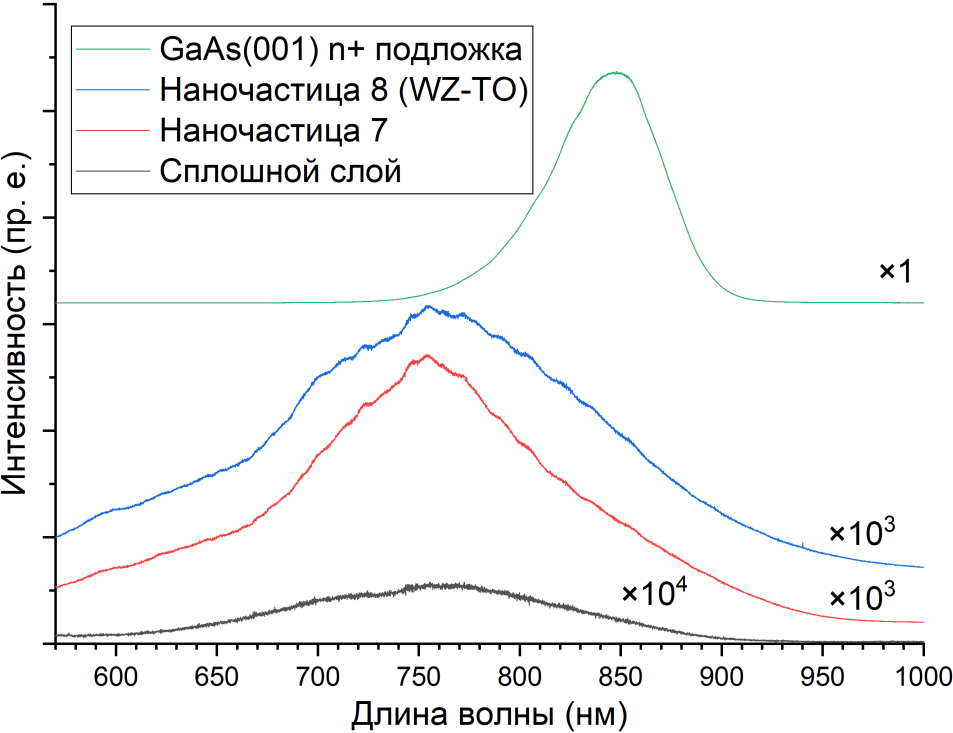
\includegraphics[width=0.6\linewidth]{Image_37} } \caption{Cпектры ФЛ от
		наночастицы~8 (с фононной модой TO-WZ), наночастицы~7, сплошного слоя и
		подложки GaAs(001)~n+ для сравнения, снятые при комнатной
температуре}\label{fig:Image_37} \end{figure}

ФЛ спектры наночастиц и сплошного слоя смещены в сторону коротких длин волн по
сравнению с объёмным GaAs \cite{Fu2004}. Сигнал ФЛ наночастиц почти на два
порядка выше по сравнению со сплошным слоем из-за меньшей плотности дефектов,
служащих центрами безызлучательной рекомбинации.

Несмотря на различия в электронной структуре WZ и ZB GaAs, в спектрах ФЛ
наночастиц с WZ включениями, снятых при комнатной температуре, явные
отличительные особенности не наблюдаются.

\section{Основные результаты главы}\label{sec:ch5/sec3}

Методом МПЭ на подложках Si(111) выращены наночастицы GaAs, исследованы
основные закономерности формирования, оптические свойства и морфология
наноструктур. Установлено, что частицы имеют огранку, образованную плоскостями
\{111\}, \{110\} и \{\(3\overline{1}1\)\}. Показано, что наночастицы
формируется по механизму ПЖК, скорость роста наночастиц непостоянна и снижается
после поглощения Ga катализатора. После чего поступающие адатомы
преимущественно встраиваются в сплошной слой, образованный планарными
островками с противоположной полярностью. Существует критическая толщина
сплошного слоя, при котором наночастицы полностью сливаются со сплошным слоем.

Увеличение молекулярного потока As может подавлять диффузию адатомов Ga, что
приводит к увеличению плотности и уменьшению критического размера наночастиц.

На спектре КРС некоторых (\(\approx 25\)\,\%) наночастиц наблюдается
дополнительный пик, соответствующий рассеянию на TO фононах решётки с WZ
структурой. Несмотря на сильное несоответствие решётки между GaAs и подложкой
Si, сдвига пиков КРС непрерывного слоя или наночастиц не наблюдается, что
указывает на релаксацию кристаллической решётки.

Сигнал ФЛ от наночастиц GaAs при комнатной температуре имеет на два порядка
более высокую интенсивность, чем у сигнала ФЛ от сплошного слоя, и смёщен в
более коротковолновую область по сравнению с объёмным материалом.

\FloatBarrier
